
\section{Robustness checks and implementation details for the simulations in Section \ref{sec-sim}}\label{sec-supp-sim}


\subsection*{Implementation of SiZer in Section \ref{subsec-sim-multiscale}}


\textcolor{red}{The SiZer methods in Section \ref{subsec-sim-multiscale} are implemented as follows:}
\begin{enumerate}[leftmargin=0.7cm,label=(\alph*)]

\item Computation of the grid $\mathcal{G}_T^*$:

To start with, we compute the variance of $\bar{Y} = T^{-1} \sum_{t=1}^T Y_{t,T}$, which is given by
\[ \var(\bar{Y}) = \frac{\gamma_\varepsilon(0)}{T} + \frac{2}{T} \sum_{k = 1}^{T-1} \Big(1 - \frac{k}{T}\Big)\gamma_\varepsilon(k). \]
Since the autocovariance function $\gamma_{\varepsilon}(\cdot)$ is known by assumption, we can calculate the value of $\var(\bar{Y})$ by using the formula $\gamma_\varepsilon(k) = \nu^2 a_1^{|k|} / (1 - a_1^2)$ together with the true para\-meters $a_1$ and $\nu^2 = \ex[\eta_t^2]$. We next compute 
\[ T^* = \frac{\gamma_\varepsilon(0)}{\var(\bar{Y})}, \]
which can be interpreted as a measure of information in the data. \textcolor{red}{For each point $(u,h) \in \mathcal{G}_T$}, we finally calculate the effective sample size for dependent data 
\[ \text{ESS}^*(u, h) = \frac{T^*}{T} \frac{\sum_{t=1}^T K_h(t/T - u)}{K_h(0)} \]
with $K_h(v) = h^{-1} K(v/h)$ and set $\mathcal{G}_T^* = \{ (u,h) \in \mathcal{G}_T: \text{ESS}^*(u, h) \ge 5 \}$. 

\item Computation of the local linear estimators and their standard deviations: 

For each $(u,h) \in \mathcal{G}_T^*$, we compute a standard local linear estimator $\widehat{m}^\prime_h(u)$ of the derivative $m^\prime(u)$ together with its standard deviation $\text{sd}(\widehat{m}^\prime_h(u))$. The latter is given by $\text{sd}(\widehat{m}^\prime_h(u)) = \{ \var(\widehat{m}^\prime_h(u)) \}^{1/2}$, where $\var(\widehat{m}^\prime_h(u)) = e^\top V e$ with $e = (\begin{matrix} 0 & 1 \end{matrix})^\top$ and 
\[ V = (X^T W X)^{-1} (X^T \Sigma X) (X^T W X)^{-1}. \]
The matrices $X$, $W$ and $\Sigma$ are defined as follows: $\Sigma$ is a $T \times T$ matrix with the elements
\[ \Sigma_{st} = \gamma_\varepsilon(s-t) K_h\Big( \frac{s}{T} - u \Big) K_h\Big( \frac{t}{T} - u \Big), \]
$W$ is a $T \times T$ diagonal matrix with the diagonal entries $K_h(t/T-u)$ and 
\[ X =   
\begin{pmatrix}
1 & (1/T - u)   \\
1 & (2/T - u)   \\
\vdots & \vdots \\
1 & (1 - u)     \\
\end{pmatrix}. \]

\item Computation of the confidence intervals:  

For a given confidence level $\alpha$ and for each bandwidth value $h$ with $(u,h) \in \mathcal{G}_T^*$, we compute the quantile 
\[ q(h) = \Phi^{-1} \Big( \Big( 1 - \frac{\alpha}{2} \Big)^{1/(\theta g)} \Big), \]
where $\Phi$ is the distribution function of a standard normal random variable, $g$ is the number of locations $u$ in the grid $\mathcal{G}_T$, and the cluster index $\theta$ is defined on p.1519 in \cite{ParkHannigKang2009}. The confidence interval of $\widehat{m}^\prime_h(u)$ is then computed as $[\widehat{m}^\prime_h(u) - q(h) \, \text{sd}(\widehat{m}^\prime_h(u)),\widehat{m}^\prime_h(u) + q(h) \, \text{sd}(\widehat{m}^\prime_h(u))]$. 

%For each $(u,h) \in \mathcal{G}_T^*$, we compute the Gaussian quantile for the confidence level $\alpha$
%\[ q(u,h) = \Phi^{-1} \Big(\frac{1 + (1 - \alpha)^{\frac{1}{l(u, h)}}}{2}\Big), \]
%where $l(u,h) = T/\text{ESS}^*(u, h)$ and $\Phi$ is the distribution function of a standard normal random variable. The confidence interval of $\widehat{m}^\prime_h(u)$ is then computed as $[\widehat{m}^\prime_h(u) - q(u,h) \, \text{sd}(\widehat{m}^\prime_h(u)),\widehat{m}^\prime_h(u) + q(u,h) \, \text{sd}(\widehat{m}^\prime_h(u))]$. 

\end{enumerate}


\subsection*{Additional power simulations for Section \ref{subsec-sim-multiscale}}


In what follows, we compare the performance of the tests $\mathcal{T}_{\text{MS}}$, $\mathcal{T}_{\text{UC}}$, $\mathcal{T}_{\text{RW}}$ and $\mathcal{T}_{\text{SiZer}}$ when (i) $m$ is the blocks signal of \cite{DonohoJohnstone1995} which was investigated in detail in \cite{HannigMarron2006} and (ii) $m$ is the sine curve $m(u) = \sin(6\pi u)$ that was considered in \cite{ParkHannigKang2009}. In both cases, the error terms are modelled as an AR($1$) process $\varepsilon_t = a_1 \varepsilon_{t-1} + \eta_1$, where $a_1 \in\{-0.5,0.5\}$ and $\eta_t$ are i.i.d.\ normal random variables with $\ex[\eta_t] = 0$ and $\ex[\eta_t^2] = \nu^2$. In the sine example, we set $\nu^2 = ??$ for $a_1 = -0.5$ and $\nu^2 = ??$ for $a_1 = 0.5$. In the blocks example, we choose $\nu^2$ such that the AR errors $\varepsilon_t$ have the variance $\var(\varepsilon_t) = 0.1^2$, which matches the variance of the i.i.d.\ errors in the blocks example of \cite{HannigMarron2006}.
%, where the errors $\varepsilon_t$ are i.i.d.\ normal with standard deviation $0.1$. To achieve this, we choose $\nu^2$ such that our AR errors $\varepsilon_t$ have standard deviation $0.1$ as well. 
Specifically, we let $\nu^2 = ??$ for $a_1 =-0.5$ and $\nu^2 = ??$ for $a_1 = 0.5$. A plot of the blocks signal is given in the two top panels of Figure \ref{fig:sizer:blocks}. As can be seen, the signal is a piecewise constant function with several jumps. We could replace this jump function by a slightly smoothed and thus differentiable version with very steep increases and decreases. However, as this leaves the simulation results essentially unchanged, we stick to the original blocks signal.  


For both the blocks and the sine example, we simulate a representative data sample of length $T=1000$ and carry out the four tests on the simulated sample for the significance level $\alpha=0.05$.\footnote{We simply set the seed equal to $1$ when prodcuing the simulated samples. So there is no cherry-picking involved!} The results are presented by SiZer maps in Figures \ref{fig:sizer:blocks} and \ref{fig:sizer:sine} which have to be read as follows: Each pixel of the SiZer map corresponds to a location-scale point $(u,h)$, or put differently, to a time intervals $[u-h,u+h]$. The pixel ($u,h)$ is coloured blue if the test finds an increase in the trend $m$ on the interval $[u-h,u+h]$, red if the test finds a decrease and purple if the test does not reject the null hypothesis that $m$ is constant on $[u-h,u+h]$. Moreover, a pixel $(u,h)$ is coloured grey if the effective sample size $\text{ESS}^*(u,h)$ is smaller than $5$, in which case the pixel $(u,h)$ is not an element of the location-scale grid $\mathcal{G}_T^*$.


The results for the blocks example are reported in Figure \ref{fig:sizer:blocks}. The left-hand panels of subfigure (a) correspond to the case with $a_1 = -0.5$. The upper panel depicts the blocks signal with the simulated data sample in the background. The other panels show the SiZer maps produced by the four tests $\mathcal{T}_{\text{MS}}$, $\mathcal{T}_{\text{UC}}$, $\mathcal{T}_{\text{RW}}$ and $\mathcal{T}_{\text{SiZer}}$. As can be seen, the SiZer maps are fairly similar. In particular, all four tests pick up the increases and decreases (that is, the upward and downward jumps) in the signal $m$ quite accurately. The situation is somewhat different in the case with $a_1 = 0.5$, which is presented in the right-hand panels of subfigure (b). Our multiscale test detects part of the increases and decreases in $m$. However, the row-wise SiZer test is able to pin down some increases and decreases which or multiscale test cannot locate. On the other 


%Row-wise procedures are more power full than global ones: Tendentially, the SiZer plots of row-wise methods have more red and blue pixels. Hence, the row-wise procedures find more increases and decreases. However, they also tend to find more spurious increases. For example, for ??



detects more increases and decreases in $m$. On the other hand, it also find two spurious decreases, which is indicated by the small red lines on fine scales at locations $u=??$ and $u=??$. This illustrates what we have already seen in simulation exercises of Section ??: On the hand, the row-wise procedure are more powerful than the global ones. On the other hand, they find spurious increases and decreases much more often.  


The results for the sine example are shown in Figure \ref{fig:sizer:sine}. The bottom-line is similar as for the blocks example. The SiZer plots for the case with $a_1=-0.5$ are very similar for the four test, which all pick up the increases decreases iof the sine curve quite qccurately. For positive AR parameter, 



. Let us first have a look at the left-hand panels of subfigure (a) which correspond to the case with $a_1=-0.5$. The upper panel depicts the sine curve with the simulatated data sample in the background. The other panels depict the sizer map prodcued by the four tests $\mathcal{T}_{\text{MS}}$, $\mathcal{T}_{\text{UC}}$, $\mathcal{T}_{\text{RW}}$ and $\mathcal{T}_{\text{SiZer}}$. As can be seen, the SiZer maps are fairly similar for the four tests. In particular, all four tests pick up the increaes and decreases of the sine curve quite clearly. Let us now move to subfigure (b) which gives the rsults for $a_1=0.5$. Overall, the results are similar. However, whereas the two row-wise procedures pick up the increase of the sine function at the left and right end of the support $[0,1]$, the two global tests do not detect these increases. This illustrates that the global procedures have less power than the row-wise ones, which is the price to pay for being able to make rigorous confidence statements. However, the global procedures allow to make rigorous confidence statements: We can clai, with confidence $95\%$ that there is indeed an increase (decrease) in the trend $m$ on all intervals $[u-h,u+h]$ which correspond to blue (red) pixels.


  



\begin{figure}[p]
\begin{subfigure}[b]{0.475\textwidth}
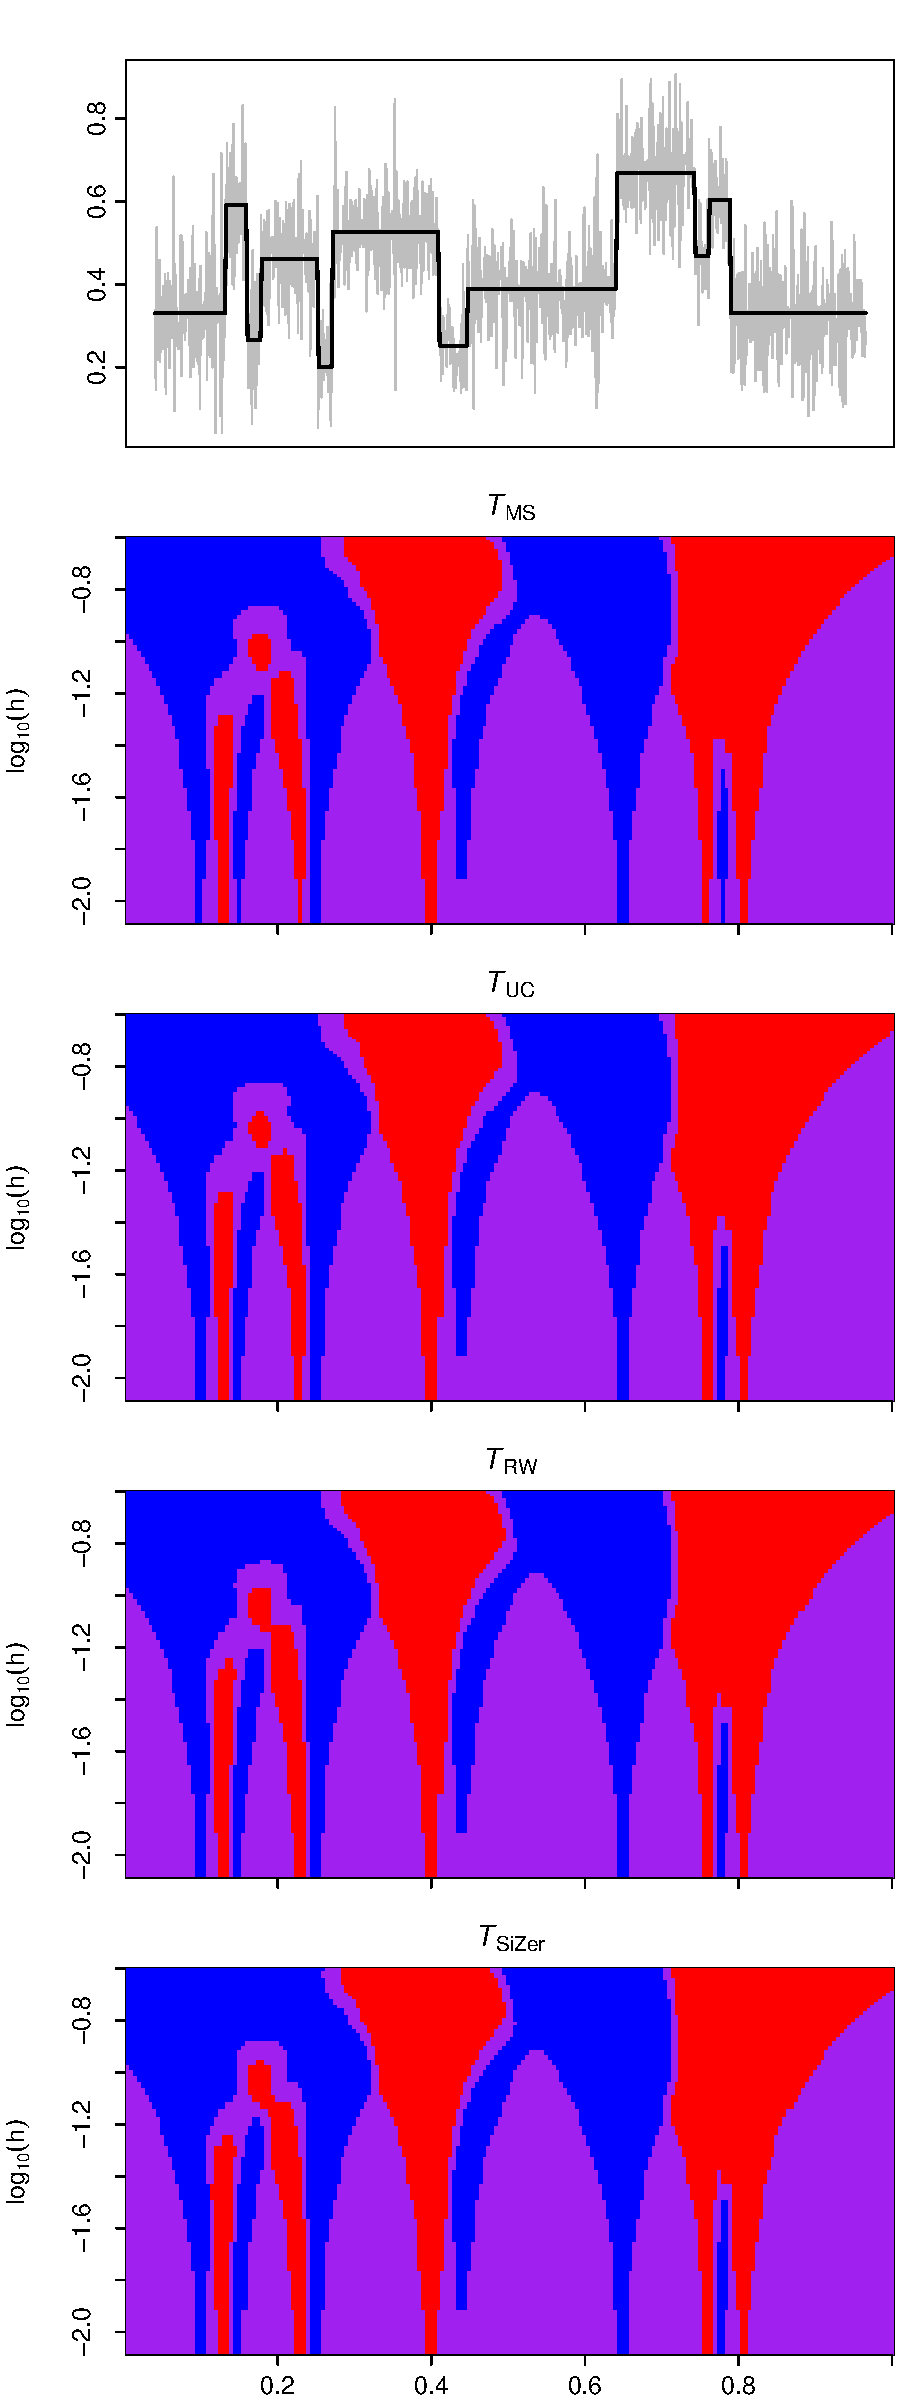
\includegraphics[width=\textwidth]{Plots/SiZer_map_T_1000_blocks_a1_-50.pdf}
\caption{$a=-0.5$}
\end{subfigure}
\hspace{0.25cm}
\begin{subfigure}[b]{0.475\textwidth}
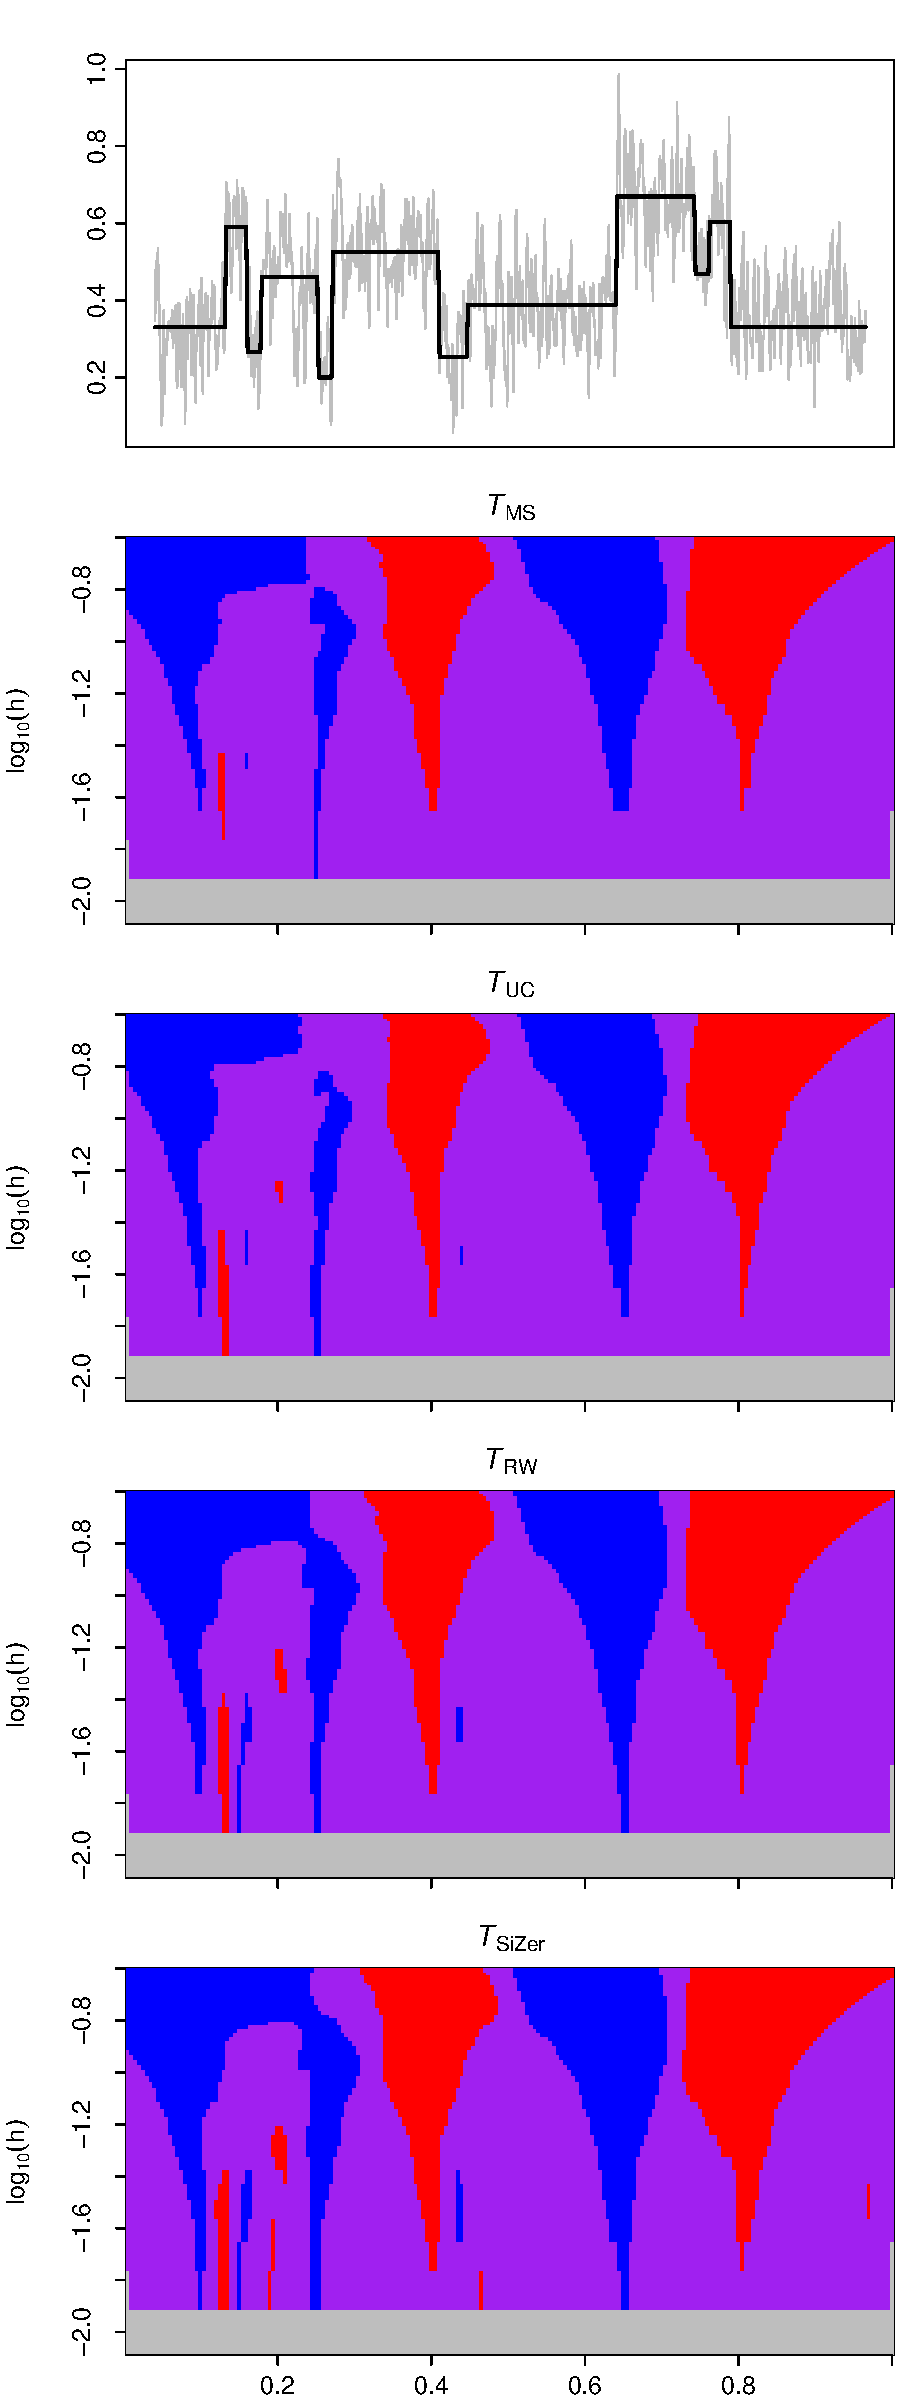
\includegraphics[width=\textwidth]{Plots/SiZer_map_T_1000_blocks_a1_50.pdf}
\caption{$a=0.5$}
\end{subfigure}
\caption{SiZer maps for the blocks example. The left-hand panels of subfigure (a) show the results for $a_1=-0.5$, the right-hand panels of subfigure (b) those for $a_1=0.5$. The two upper panels depicts the sine curve with the simulated data sample in the background.}\label{fig:sizer:blocks}
\end{figure}


\begin{figure}[p]
\begin{subfigure}[b]{0.475\textwidth}
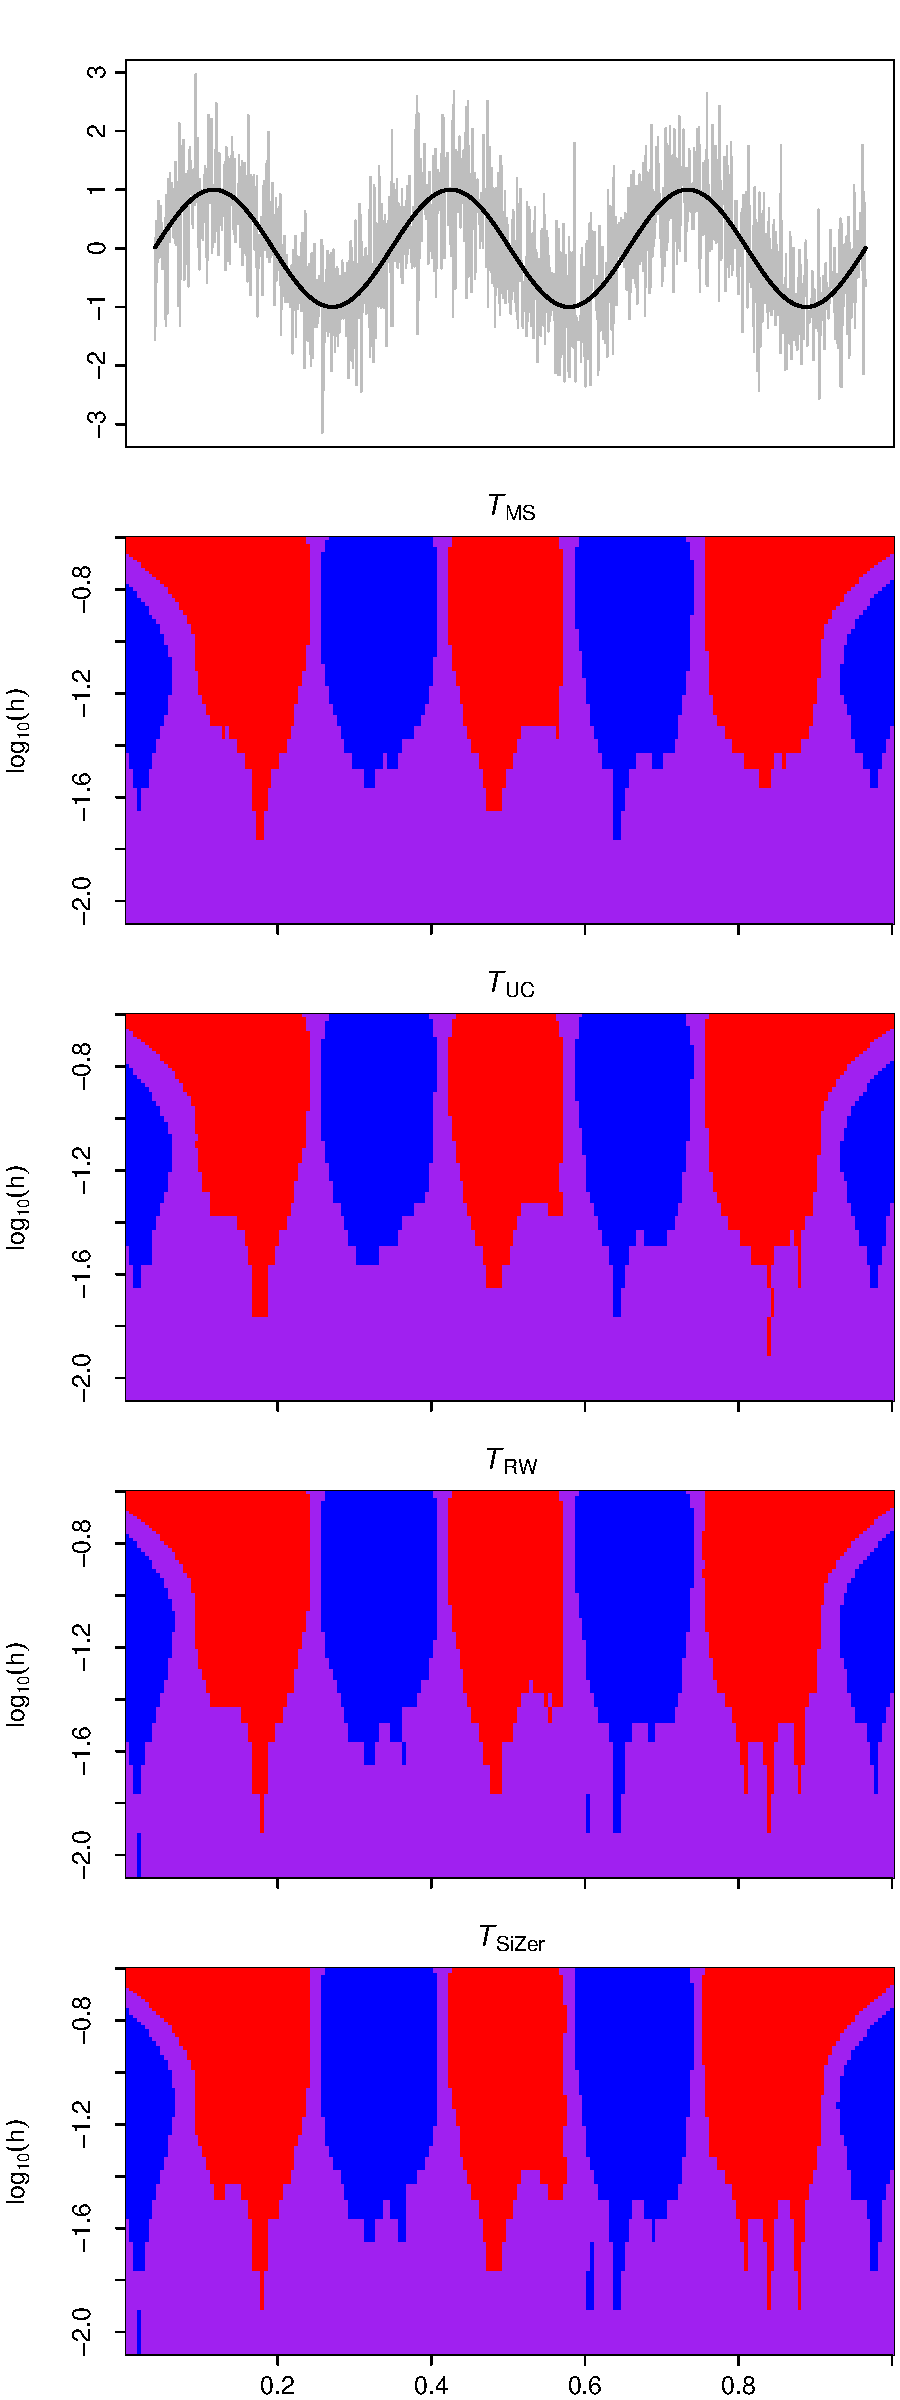
\includegraphics[width=\textwidth]{Plots/SiZer_map_T_1000_sine_a1_-50.pdf}
\caption{$a=-0.5$}
\end{subfigure}
\hspace{0.25cm}
\begin{subfigure}[b]{0.475\textwidth}
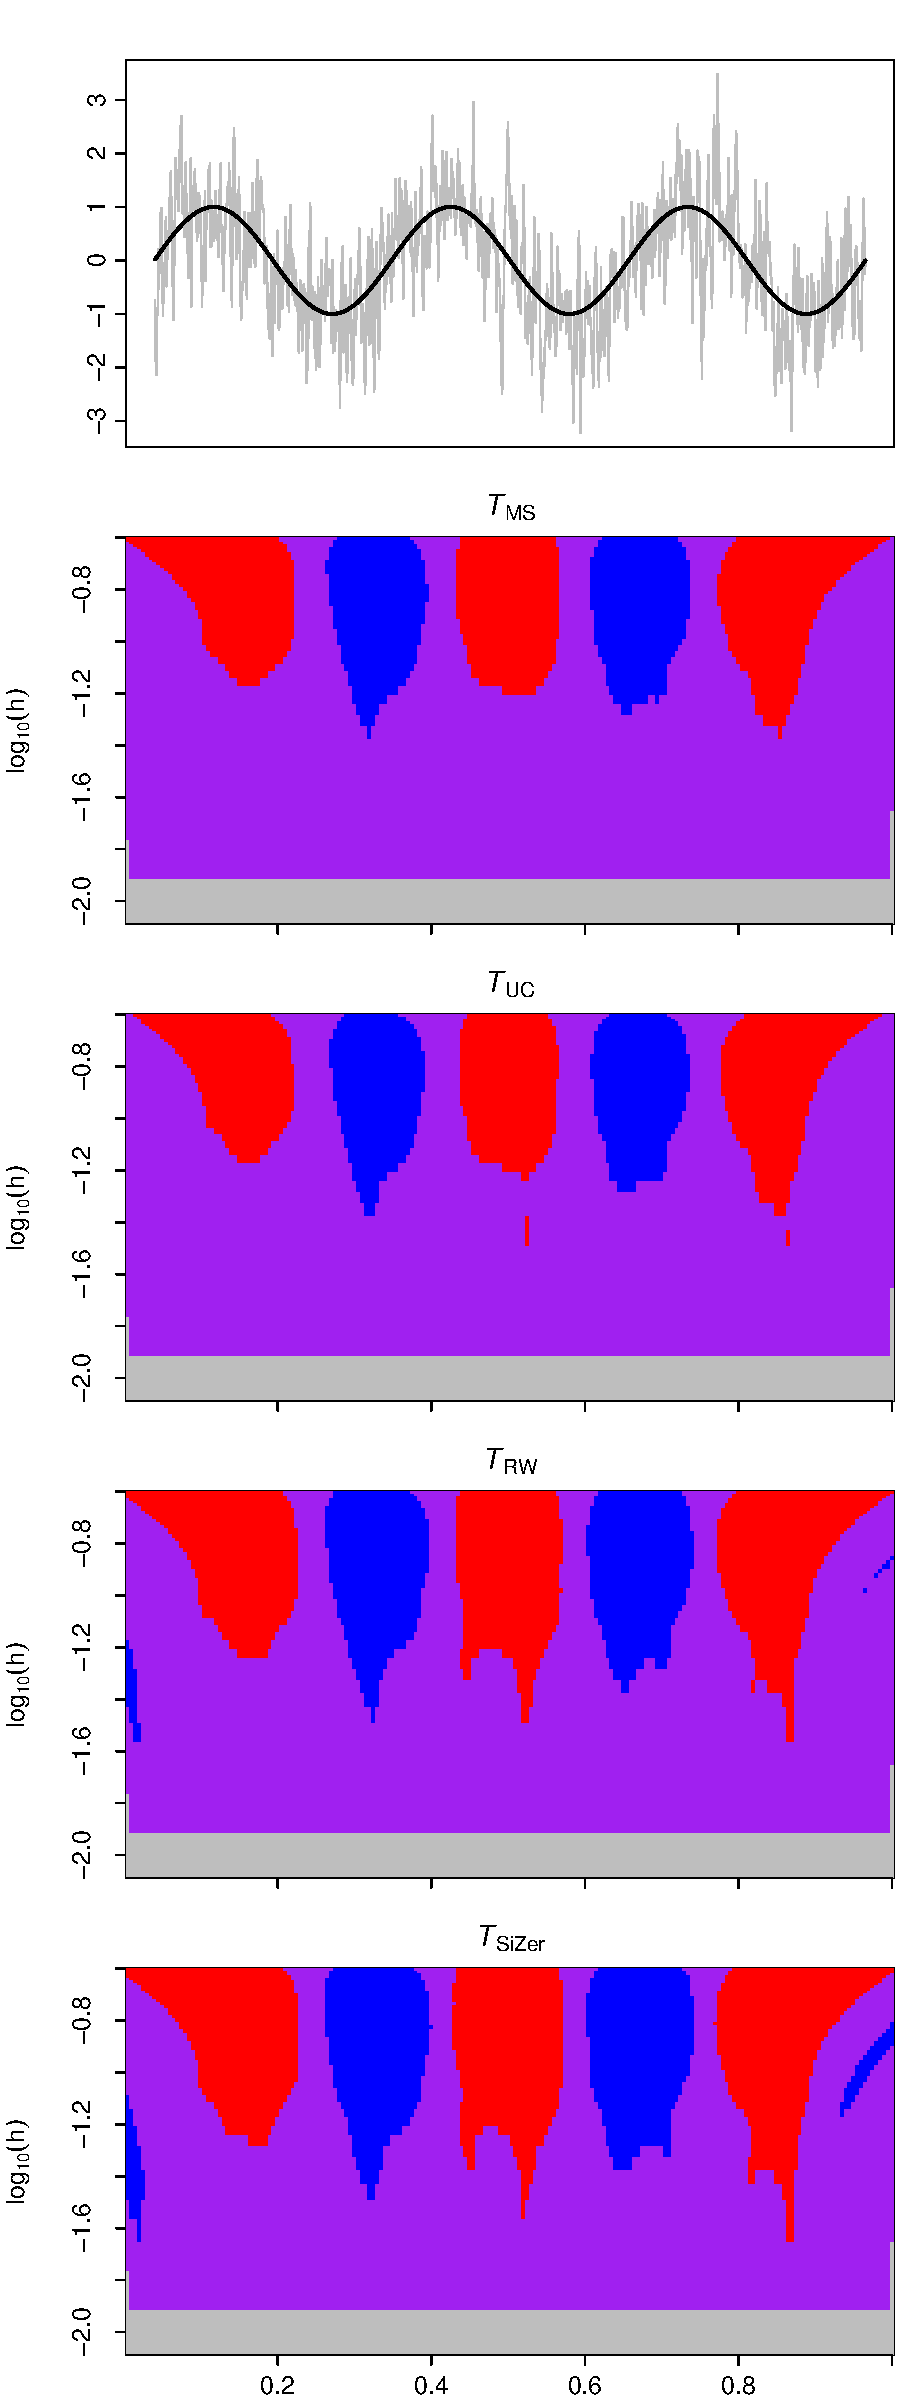
\includegraphics[width=\textwidth]{Plots/SiZer_map_T_1000_sine_a1_50.pdf}
\caption{$a=0.5$}
\end{subfigure}
\caption{SiZer maps for the sine example. The left-hand panels of subfigure (a) show the results for $a_1=-0.5$, the right-hand panels of subfigure (b) those for $a_1=0.5$. The two upper panels depicts the sine curve with the simulated data sample in the background.}\label{fig:sizer:sine}
\end{figure}  



\subsection*{Robustness checks for Section \ref{subsec-sim-lrv}}


In what follows, we carry out some robustness checks to assess how sensitive the estimators $\widehat{a}$ and $\widehat{\sigma}^2$ are to the choice of the tuning parameters $q$ and $\overline{r}$. To do so, we repeat the simulation exercises of Section \ref{subsec-sim-lrv} for different values of $q$ and $\overline{r}$. In addition, we consider different choices of the tuning parameters $(m_1,m_2)$ on which the estimators of \cite{Hall2003} depend. As in Section \ref{subsec-sim-lrv}, we choose $m_1$ and $m_2$ such that $q$ lies between these values. We thus keep the parameters $q$ and $(m_1,m_2)$ roughly comparable. 


To start with, we consider the simulation scenarios with a moderate trend ($s_\beta = 1$). The MSE values of the estimators $\widehat{a}$, $\widehat{a}_{\text{HvK}}$, $\widehat{a}_{\text{oracle}}$ and $\widehat{\sigma}^2$, $\widehat{\sigma}^2_{\text{HvK}}$, $\widehat{\sigma}^2_{\text{oracle}}$ for these scenarios are presented in Figure \ref{fig:MSE_slope1} of Section \ref{subsec-sim-lrv}. These MSEs are re-calculated in Figures \ref{fig:MSE_slope1_AR_robust} and \ref{fig:MSE_slope1_lrv_robust} for a range of different choices of $q$, $\overline{r}$ and $(m_1,m_2)$. As one can see, the MSEs in the different plots of Figures \ref{fig:MSE_slope1_AR_robust} and \ref{fig:MSE_slope1_lrv_robust} are very similar. Hence, the MSE results reported in Section \ref{subsec-sim-lrv} for the scenarios with a moderate trend appear to be fairly robust to different choices of the tuning parameters. In particular, our estimators $\widehat{a}$ and $\widehat{\sigma}^2$ seem to be quite insensitive to the choice of tuning parameters, at least as far as their MSEs are concerned.


We next turn to the simulation designs with a pronounced trend ($s_\beta = 10$). The MSE values of the estimators in these scenarios are reported in Figure \ref{fig:MSE_slope10} of Section \ref{subsec-sim-lrv}. Analogously as before, we re-calculate these MSEs for different tuning parameters in Figures \ref{fig:MSE_slope10_AR_robust}--\ref{fig:MSE_slope10_lrv_robust}. Figure \ref{fig:MSE_slope10_AR_zoom_robust} is a zoomed-in version of Figure \ref{fig:MSE_slope10_AR_robust} which is added for better visibility. As can be seen, our estimators appear to be barely influenced by the choice of $q$. However, the MSE values become somewhat larger when $\overline{r}$ is chosen bigger. This is of course not very surprising: The main reason why the estimator $\widehat{a}$ works well in the presence of a strong trend is that it is only based on differences of small orders. If we increase $\overline{r}$, we use larger differences to compute $\widehat{a}$, which results in not eliminating the trend $m$ appropriately any more. This becomes visible in somewhat larger MSE values. Nevertheless, overall, our estimators appear not to be strongly influenced by the choice of tuning parameters (in terms of MSE) as long as these are chosen within reasonable bounds. 


\begin{figure}[h!]
\begin{subfigure}[b]{0.45\textwidth}
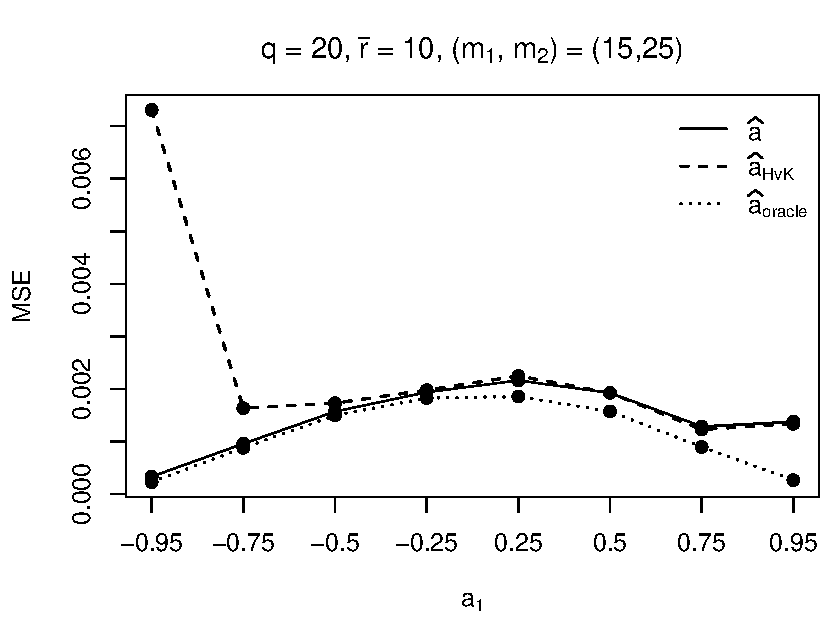
\includegraphics[width=\textwidth]{Plots/Robustness/MSE_a1_T=500_slope=1_(q,r,M1,M2)=(20,10,15,25).pdf}
\end{subfigure}
\hspace{0.25cm}
\begin{subfigure}[b]{0.45\textwidth}
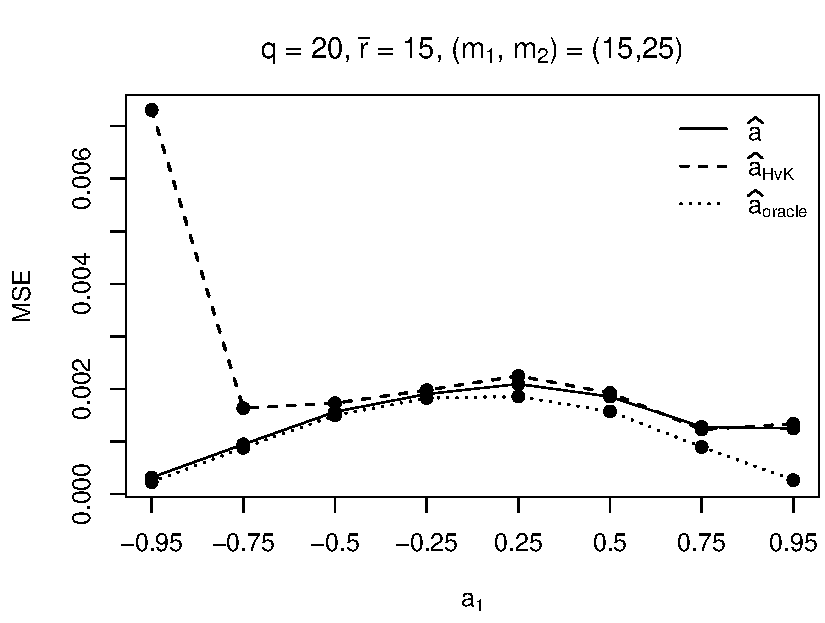
\includegraphics[width=\textwidth]{Plots/Robustness/MSE_a1_T=500_slope=1_(q,r,M1,M2)=(20,15,15,25).pdf}
\end{subfigure}

\begin{subfigure}[b]{0.45\textwidth}
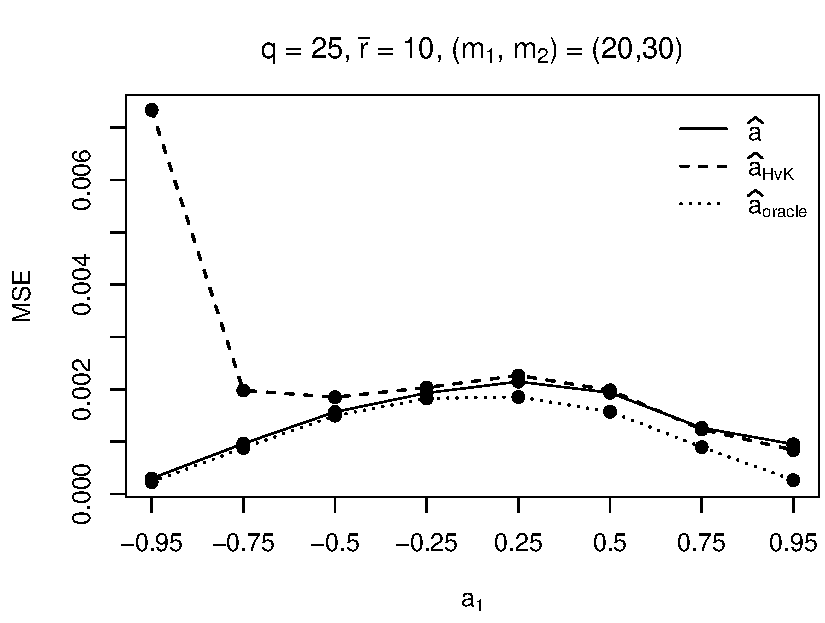
\includegraphics[width=\textwidth]{Plots/Robustness/MSE_a1_T=500_slope=1_(q,r,M1,M2)=(25,10,20,30).pdf}
\end{subfigure}
\hspace{0.25cm}
\begin{subfigure}[b]{0.45\textwidth}
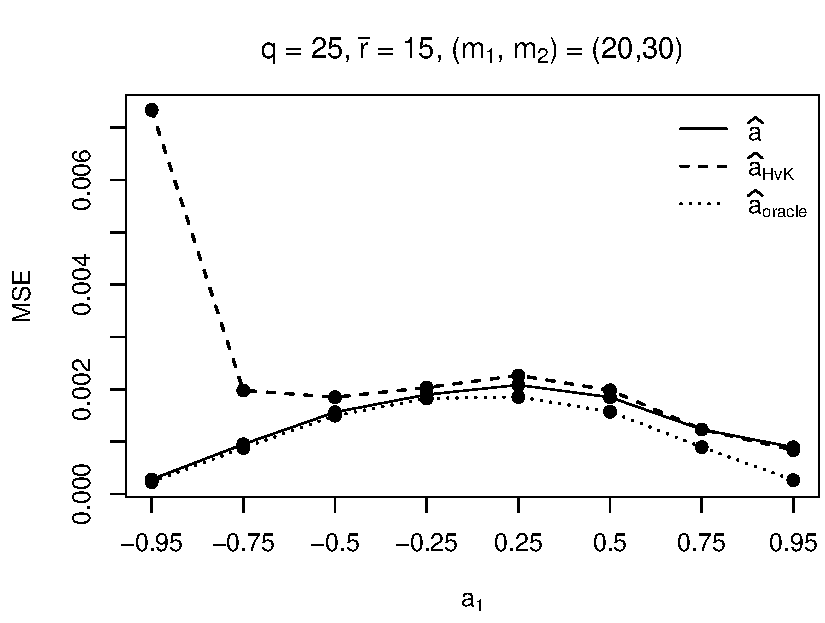
\includegraphics[width=\textwidth]{Plots/Robustness/MSE_a1_T=500_slope=1_(q,r,M1,M2)=(25,15,20,30).pdf}
\end{subfigure}

\begin{subfigure}[b]{0.45\textwidth}
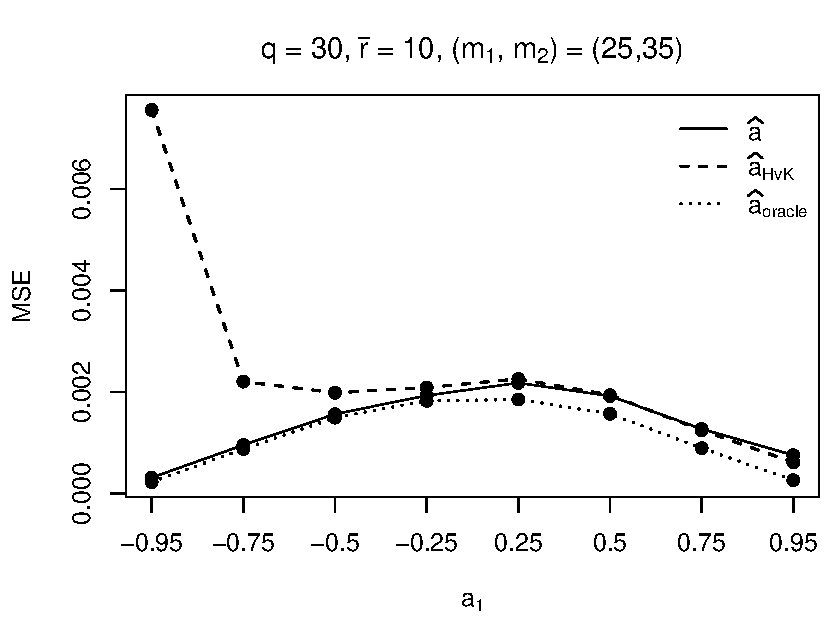
\includegraphics[width=\textwidth]{Plots/Robustness/MSE_a1_T=500_slope=1_(q,r,M1,M2)=(30,10,25,35).pdf}
\end{subfigure}
\hspace{0.25cm}
\begin{subfigure}[b]{0.45\textwidth}
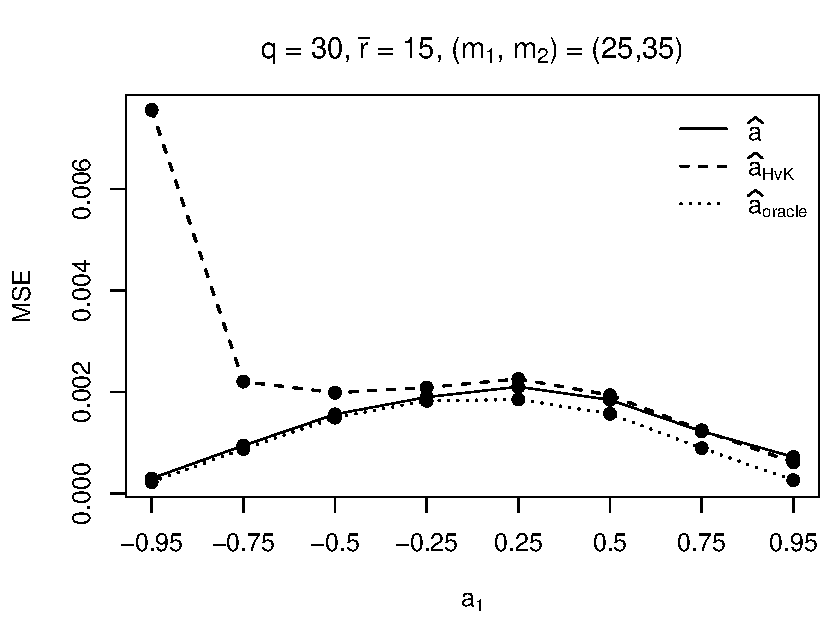
\includegraphics[width=\textwidth]{Plots/Robustness/MSE_a1_T=500_slope=1_(q,r,M1,M2)=(30,15,25,35).pdf}
\end{subfigure}

\begin{subfigure}[b]{0.45\textwidth}
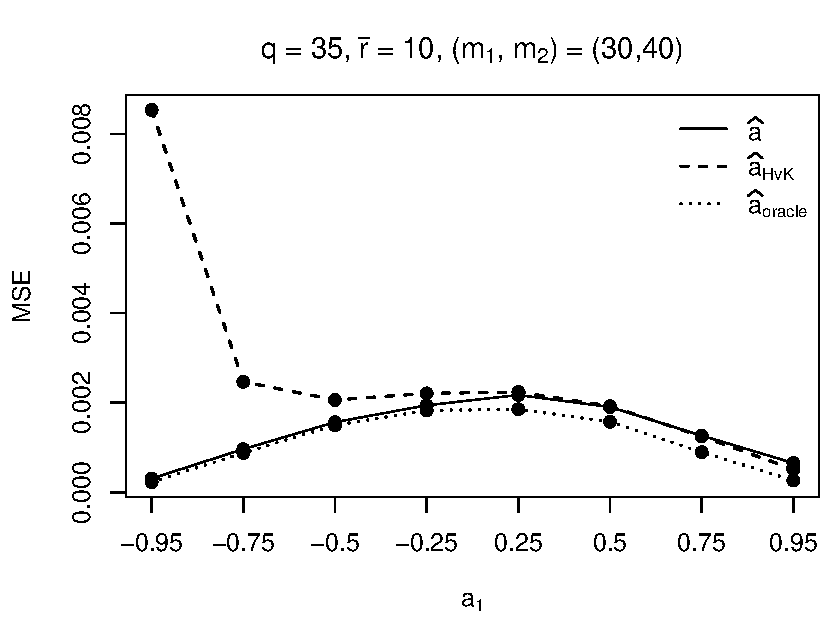
\includegraphics[width=\textwidth]{Plots/Robustness/MSE_a1_T=500_slope=1_(q,r,M1,M2)=(35,10,30,40).pdf}
\end{subfigure}
\hspace{0.25cm}
\begin{subfigure}[b]{0.45\textwidth}
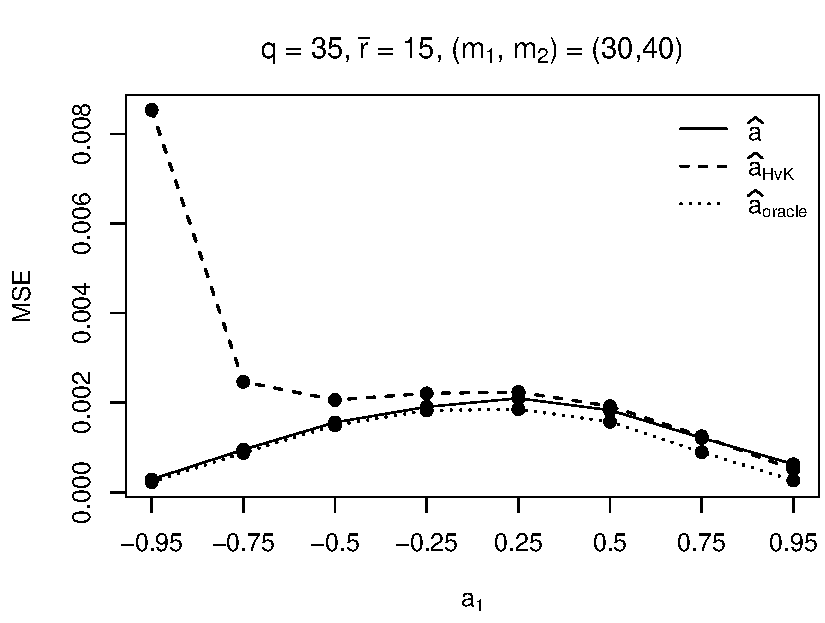
\includegraphics[width=\textwidth]{Plots/Robustness/MSE_a1_T=500_slope=1_(q,r,M1,M2)=(35,15,30,40).pdf}
\end{subfigure}
\caption{MSE values for the estimators $\widehat{a}$, $\widehat{a}_{\text{HvK}}$ and $\widehat{a}_{\text{oracle}}$ in the scenario with a moderate trend ($s_\beta=1$).}\label{fig:MSE_slope1_AR_robust} 
\end{figure}


\begin{figure}[p]
\begin{subfigure}[b]{0.45\textwidth}
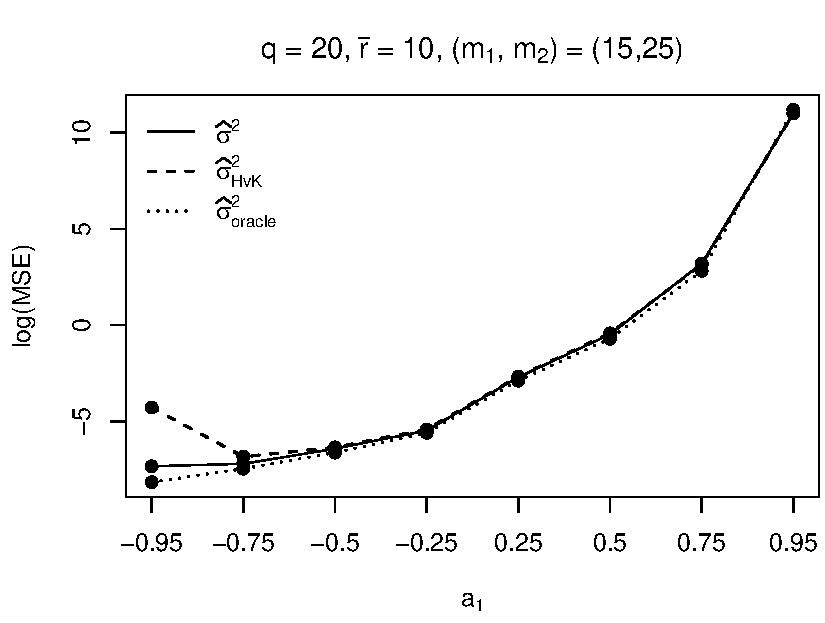
\includegraphics[width=\textwidth]{Plots/Robustness/MSE_lrv_T=500_slope=1_(q,r,M1,M2)=(20,10,15,25).pdf}
\end{subfigure}
\hspace{0.25cm}
\begin{subfigure}[b]{0.45\textwidth}
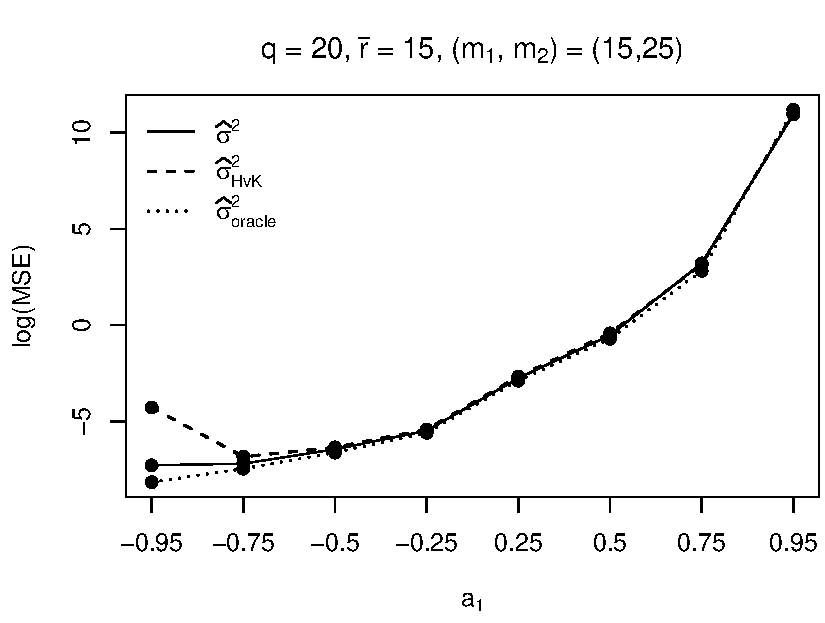
\includegraphics[width=\textwidth]{Plots/Robustness/MSE_lrv_T=500_slope=1_(q,r,M1,M2)=(20,15,15,25).pdf}
\end{subfigure}

\begin{subfigure}[b]{0.45\textwidth}
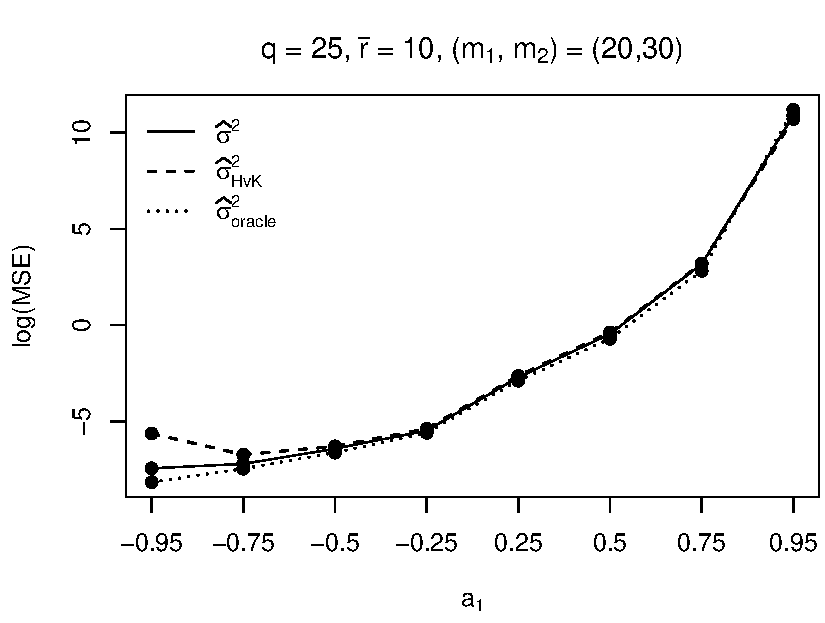
\includegraphics[width=\textwidth]{Plots/Robustness/MSE_lrv_T=500_slope=1_(q,r,M1,M2)=(25,10,20,30).pdf}
\end{subfigure}
\hspace{0.25cm}
\begin{subfigure}[b]{0.45\textwidth}
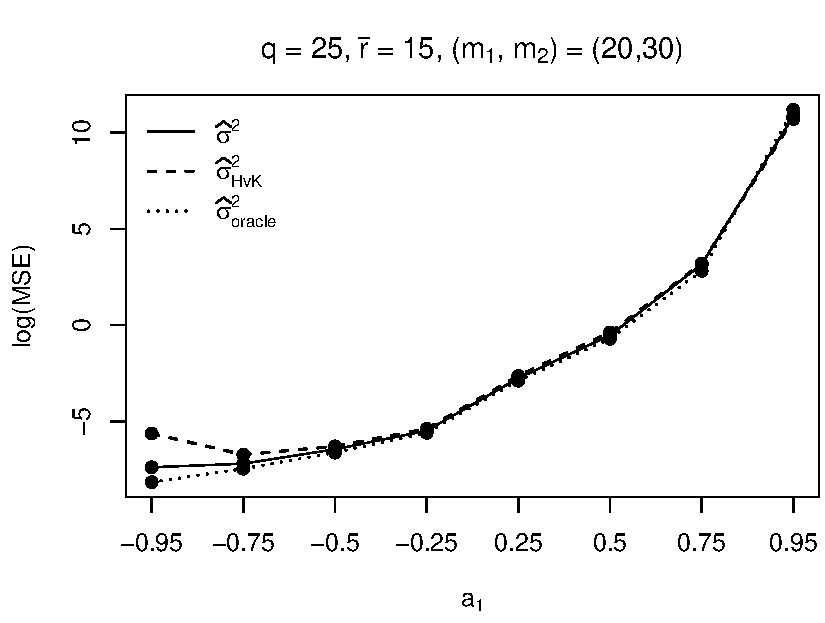
\includegraphics[width=\textwidth]{Plots/Robustness/MSE_lrv_T=500_slope=1_(q,r,M1,M2)=(25,15,20,30).pdf}
\end{subfigure}

\begin{subfigure}[b]{0.45\textwidth}
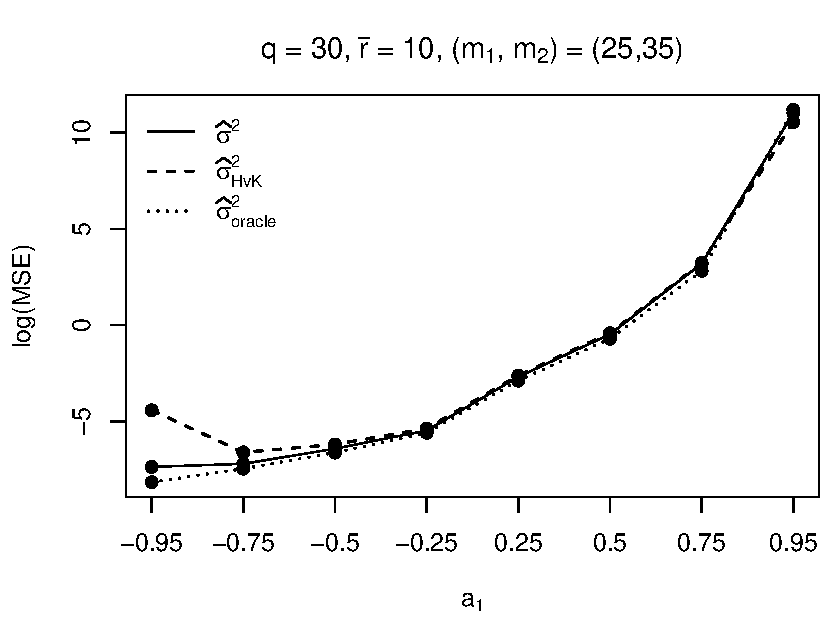
\includegraphics[width=\textwidth]{Plots/Robustness/MSE_lrv_T=500_slope=1_(q,r,M1,M2)=(30,10,25,35).pdf}
\end{subfigure}
\hspace{0.25cm}
\begin{subfigure}[b]{0.45\textwidth}
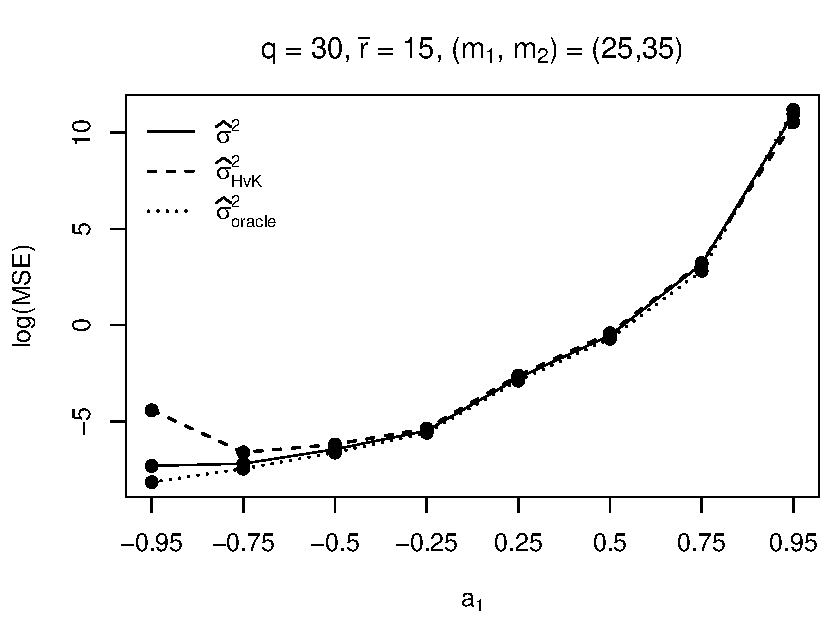
\includegraphics[width=\textwidth]{Plots/Robustness/MSE_lrv_T=500_slope=1_(q,r,M1,M2)=(30,15,25,35).pdf}
\end{subfigure}

\begin{subfigure}[b]{0.45\textwidth}
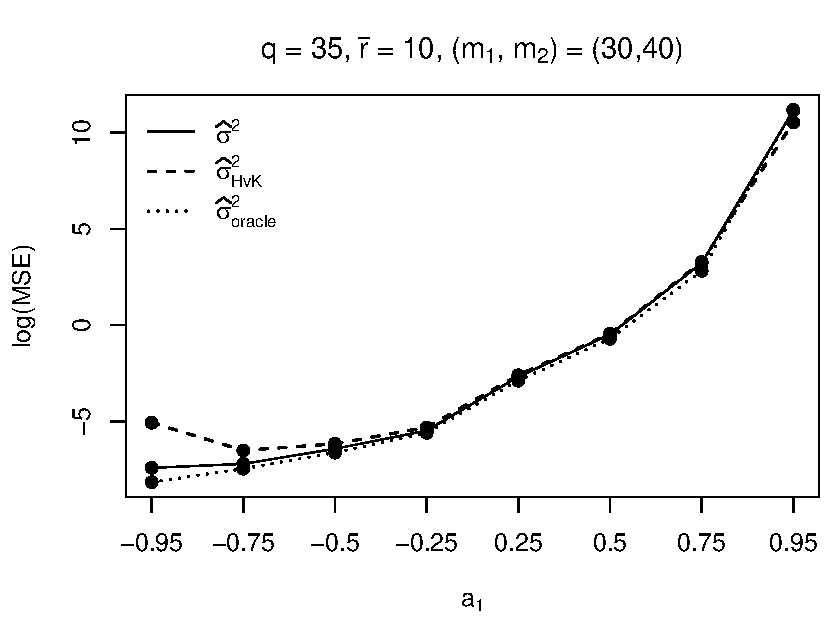
\includegraphics[width=\textwidth]{Plots/Robustness/MSE_lrv_T=500_slope=1_(q,r,M1,M2)=(35,10,30,40).pdf}
\end{subfigure}
\hspace{0.25cm}
\begin{subfigure}[b]{0.45\textwidth}
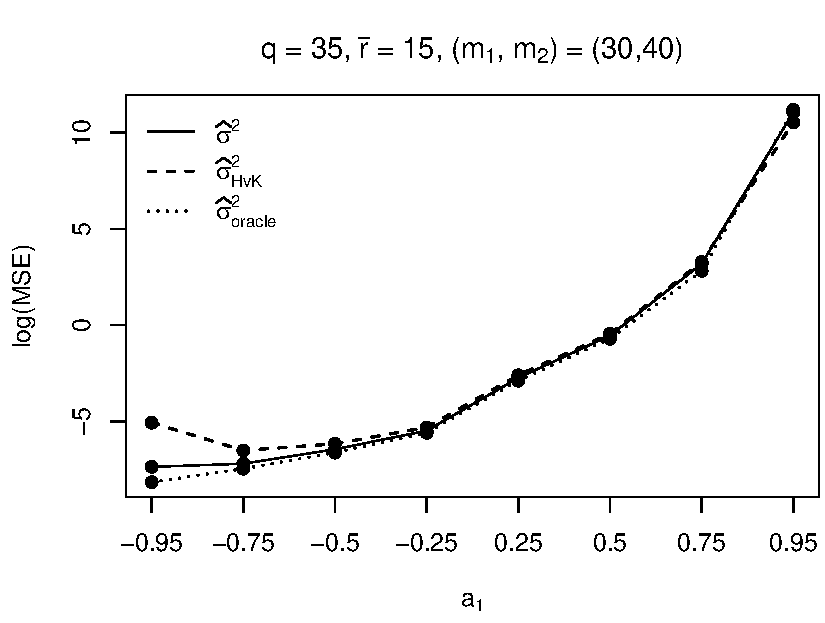
\includegraphics[width=\textwidth]{Plots/Robustness/MSE_lrv_T=500_slope=1_(q,r,M1,M2)=(35,15,30,40).pdf}
\end{subfigure}
\caption{Logarithmic MSE values for the estimators $\widehat{\sigma}^2$, $\widehat{\sigma}^2_{\text{HvK}}$ and $\widehat{\sigma}^2_{\text{oracle}}$ in the scenario with a moderate trend ($s_\beta=1$).}\label{fig:MSE_slope1_lrv_robust}
\end{figure}


\begin{figure}[p]
\begin{subfigure}[b]{0.45\textwidth}
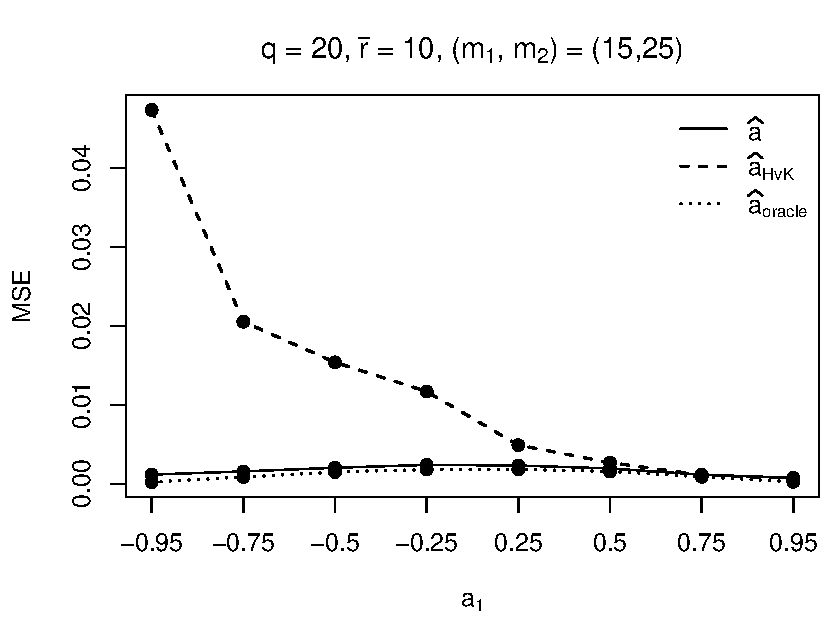
\includegraphics[width=\textwidth]{Plots/Robustness/MSE_a1_T=500_slope=10_(q,r,M1,M2)=(20,10,15,25).pdf}
\end{subfigure}
\hspace{0.25cm}
\begin{subfigure}[b]{0.45\textwidth}
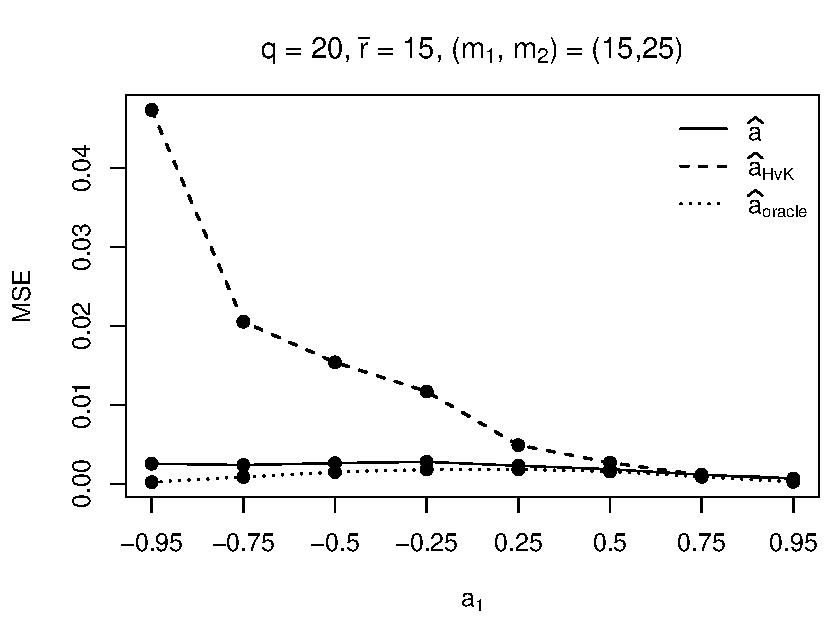
\includegraphics[width=\textwidth]{Plots/Robustness/MSE_a1_T=500_slope=10_(q,r,M1,M2)=(20,15,15,25).pdf}
\end{subfigure}

\begin{subfigure}[b]{0.45\textwidth}
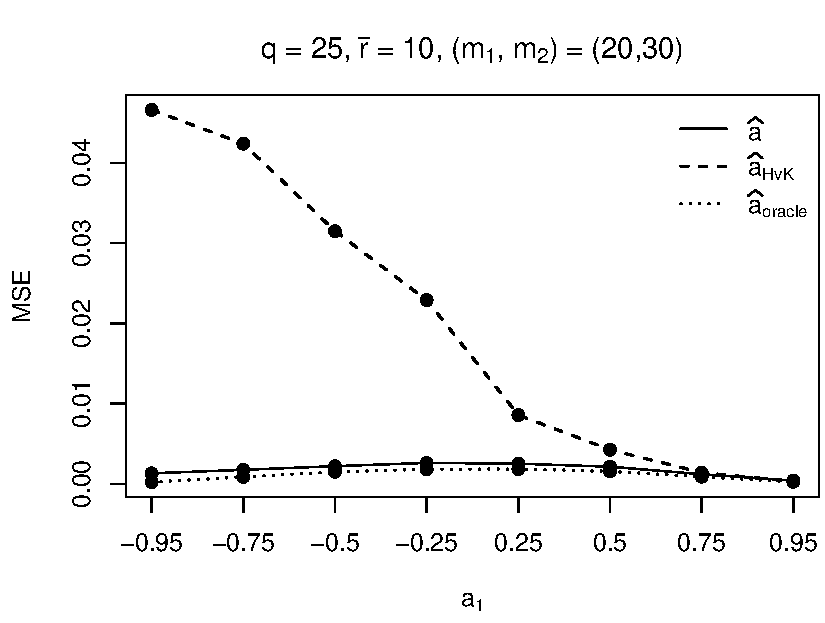
\includegraphics[width=\textwidth]{Plots/Robustness/MSE_a1_T=500_slope=10_(q,r,M1,M2)=(25,10,20,30).pdf}
\end{subfigure}
\hspace{0.25cm}
\begin{subfigure}[b]{0.45\textwidth}
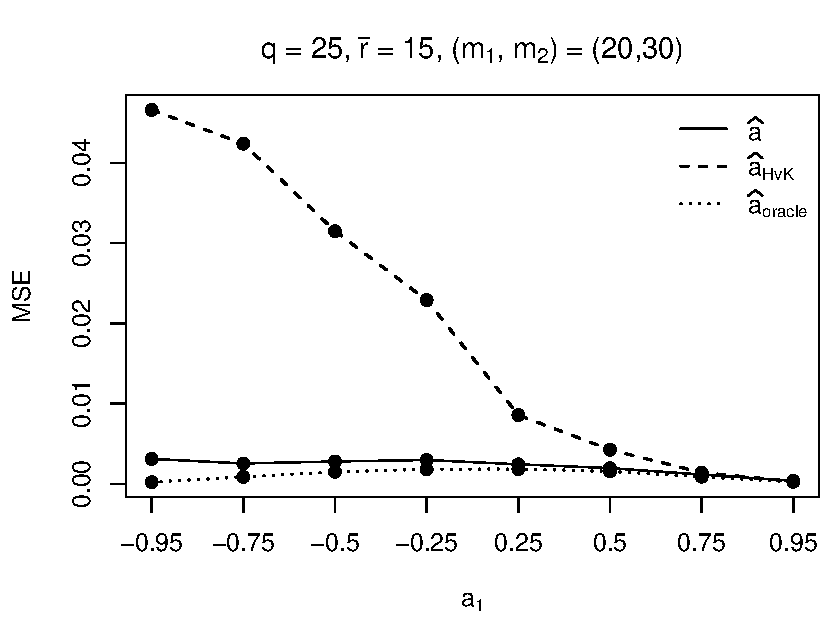
\includegraphics[width=\textwidth]{Plots/Robustness/MSE_a1_T=500_slope=10_(q,r,M1,M2)=(25,15,20,30).pdf}
\end{subfigure}

\begin{subfigure}[b]{0.45\textwidth}
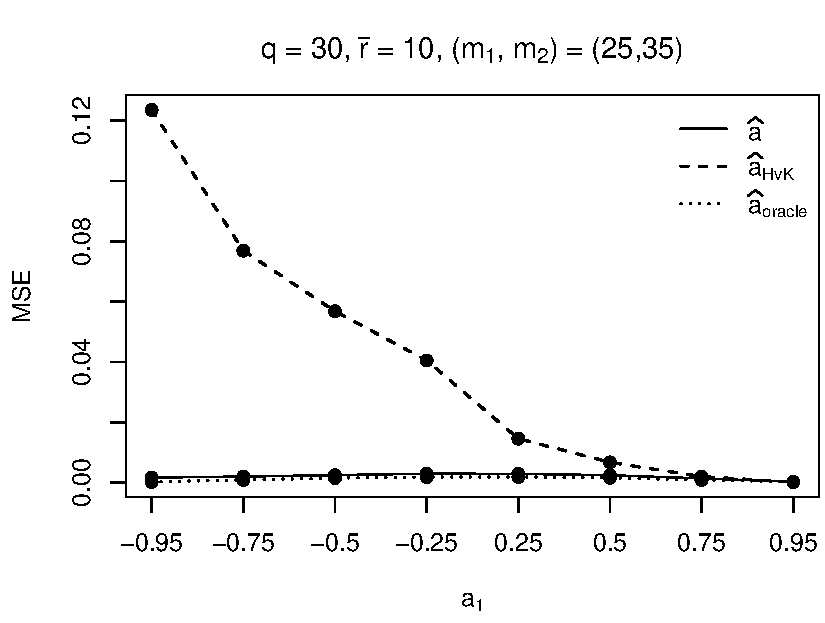
\includegraphics[width=\textwidth]{Plots/Robustness/MSE_a1_T=500_slope=10_(q,r,M1,M2)=(30,10,25,35).pdf}
\end{subfigure}
\hspace{0.25cm}
\begin{subfigure}[b]{0.45\textwidth}
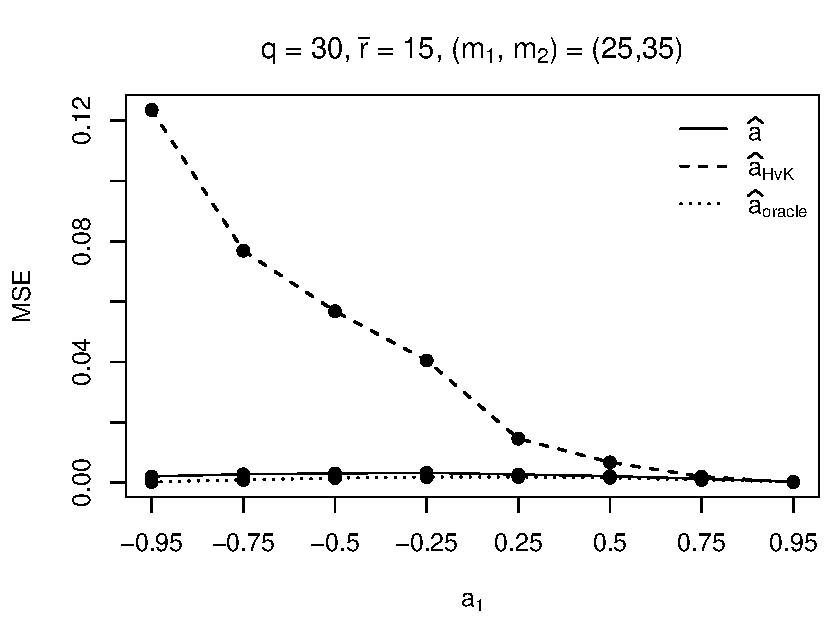
\includegraphics[width=\textwidth]{Plots/Robustness/MSE_a1_T=500_slope=10_(q,r,M1,M2)=(30,15,25,35).pdf}
\end{subfigure}

\begin{subfigure}[b]{0.45\textwidth}
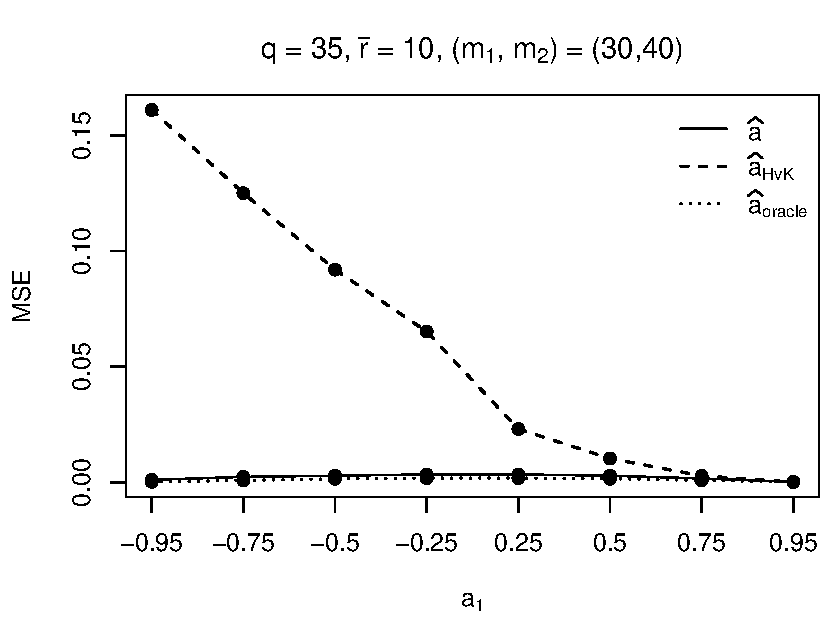
\includegraphics[width=\textwidth]{Plots/Robustness/MSE_a1_T=500_slope=10_(q,r,M1,M2)=(35,10,30,40).pdf}
\end{subfigure}
\hspace{0.25cm}
\begin{subfigure}[b]{0.45\textwidth}
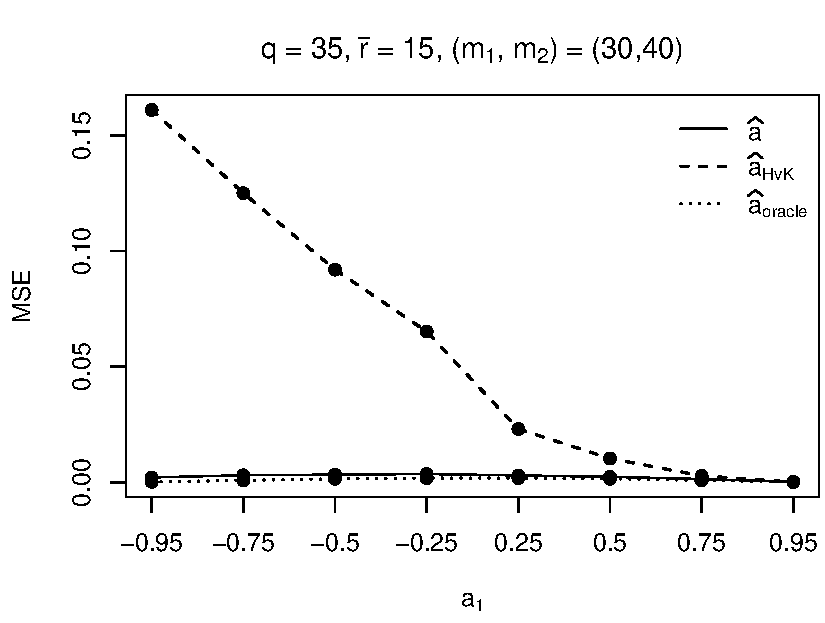
\includegraphics[width=\textwidth]{Plots/Robustness/MSE_a1_T=500_slope=10_(q,r,M1,M2)=(35,15,30,40).pdf}
\end{subfigure}
\caption{MSE values for the estimators $\widehat{a}$, $\widehat{a}_{\text{HvK}}$ and $\widehat{a}_{\text{oracle}}$ in the scenario with a pronounced trend ($s_\beta=10$).}\label{fig:MSE_slope10_AR_robust} 
\end{figure}


\begin{figure}[p]
\begin{subfigure}[b]{0.45\textwidth}
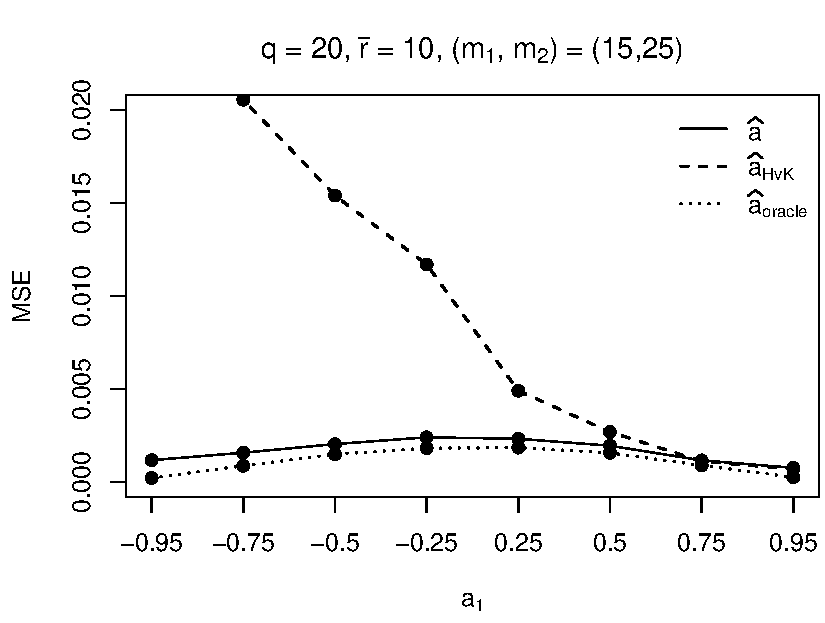
\includegraphics[width=\textwidth]{Plots/Robustness/MSE_a1_zoomed_T=500_slope=10_(q,r,M1,M2)=(20,10,15,25).pdf}
\end{subfigure}
\hspace{0.25cm}
\begin{subfigure}[b]{0.45\textwidth}
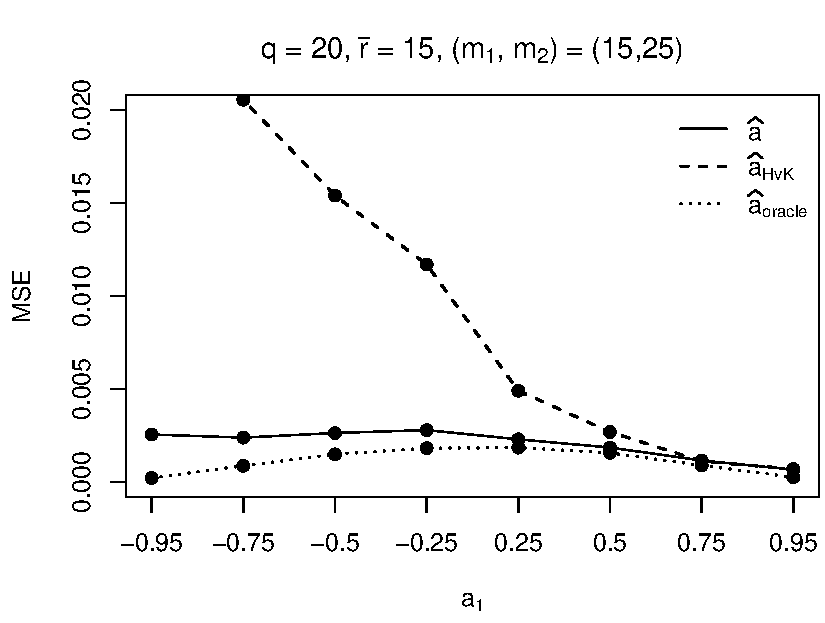
\includegraphics[width=\textwidth]{Plots/Robustness/MSE_a1_zoomed_T=500_slope=10_(q,r,M1,M2)=(20,15,15,25).pdf}
\end{subfigure}

\begin{subfigure}[b]{0.45\textwidth}
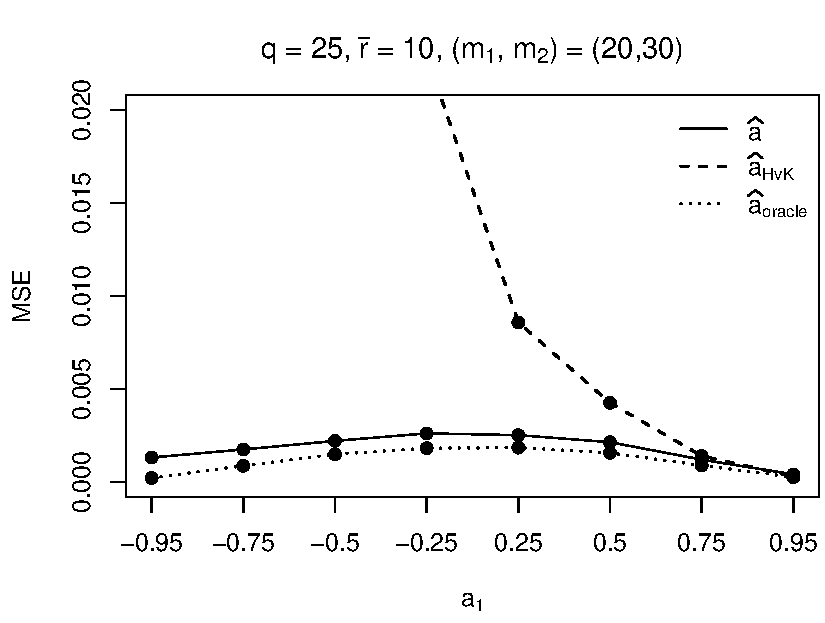
\includegraphics[width=\textwidth]{Plots/Robustness/MSE_a1_zoomed_T=500_slope=10_(q,r,M1,M2)=(25,10,20,30).pdf}
\end{subfigure}
\hspace{0.25cm}
\begin{subfigure}[b]{0.45\textwidth}
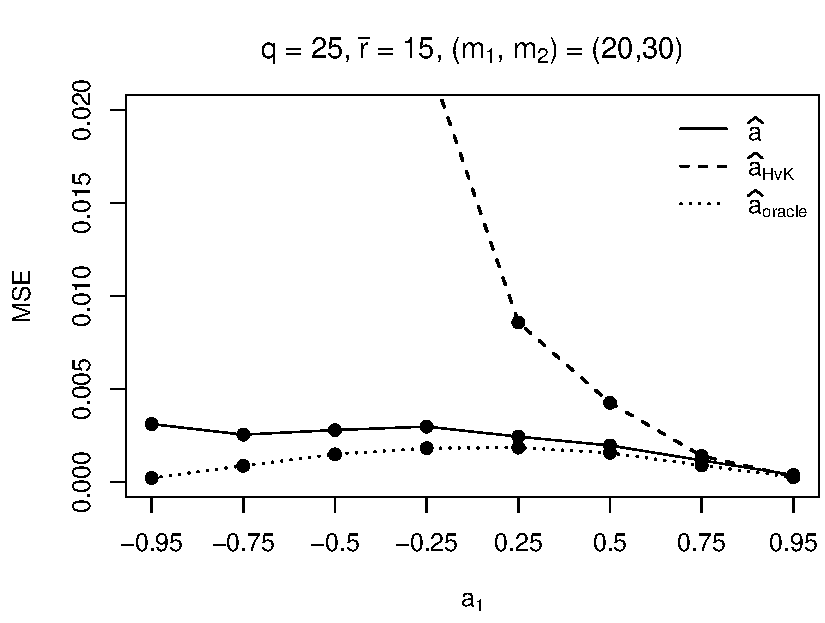
\includegraphics[width=\textwidth]{Plots/Robustness/MSE_a1_zoomed_T=500_slope=10_(q,r,M1,M2)=(25,15,20,30).pdf}
\end{subfigure}

\begin{subfigure}[b]{0.45\textwidth}
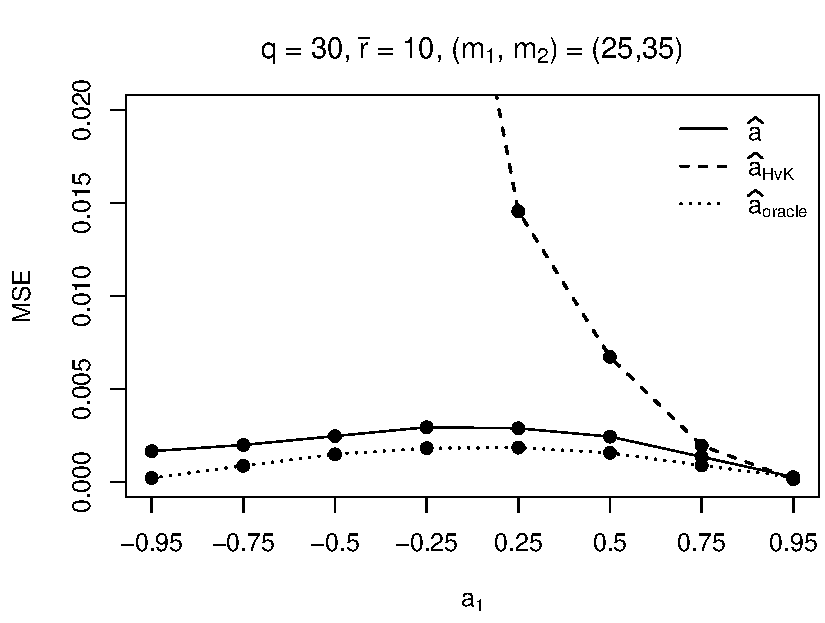
\includegraphics[width=\textwidth]{Plots/Robustness/MSE_a1_zoomed_T=500_slope=10_(q,r,M1,M2)=(30,10,25,35).pdf}
\end{subfigure}
\hspace{0.25cm}
\begin{subfigure}[b]{0.45\textwidth}
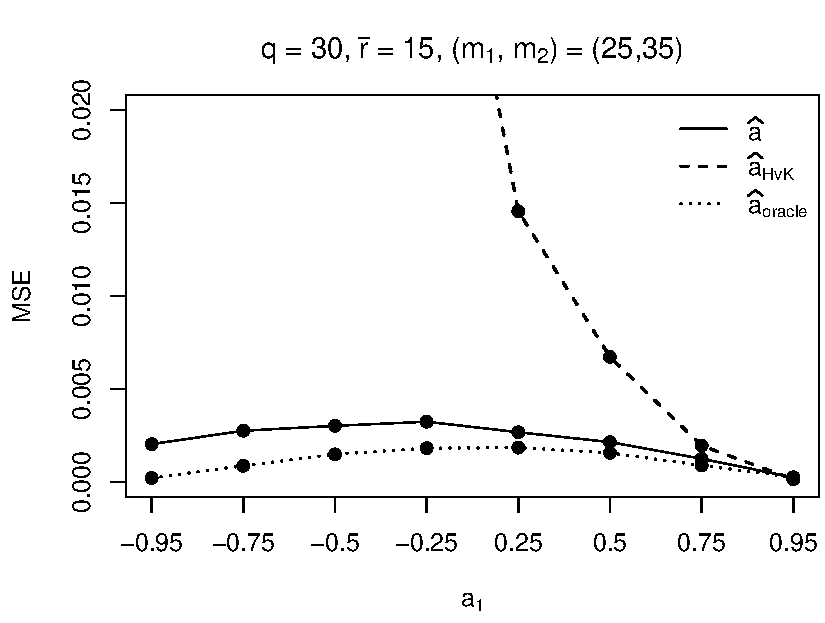
\includegraphics[width=\textwidth]{Plots/Robustness/MSE_a1_zoomed_T=500_slope=10_(q,r,M1,M2)=(30,15,25,35).pdf}
\end{subfigure}

\begin{subfigure}[b]{0.45\textwidth}
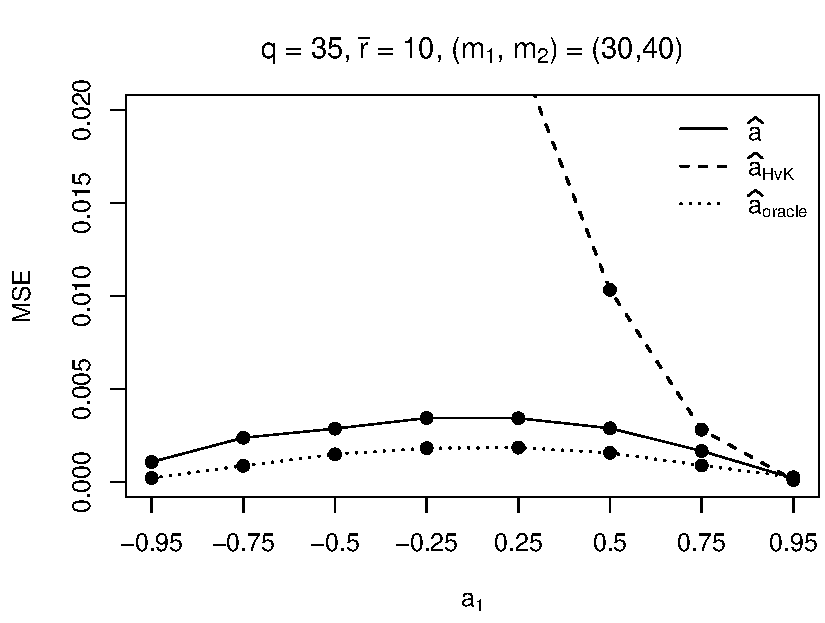
\includegraphics[width=\textwidth]{Plots/Robustness/MSE_a1_zoomed_T=500_slope=10_(q,r,M1,M2)=(35,10,30,40).pdf}
\end{subfigure}
\hspace{0.25cm}
\begin{subfigure}[b]{0.45\textwidth}
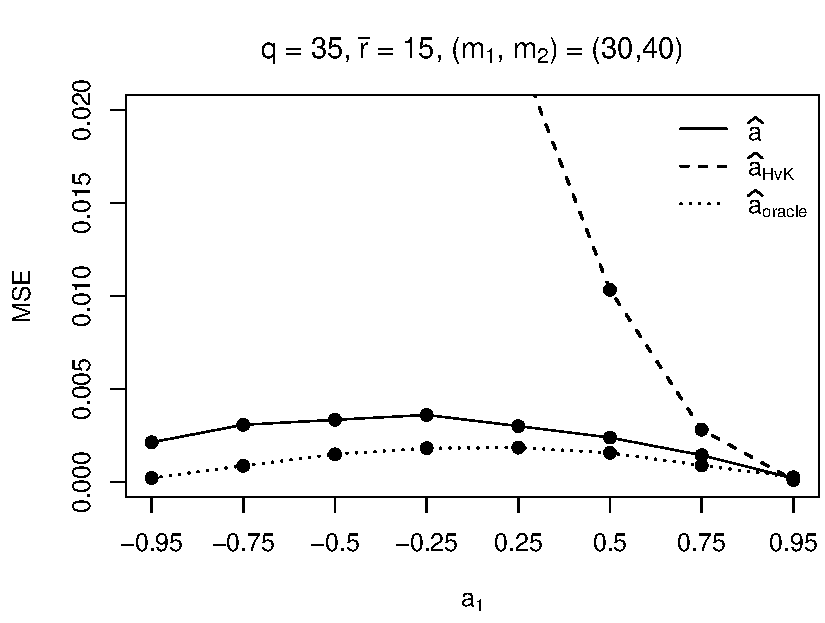
\includegraphics[width=\textwidth]{Plots/Robustness/MSE_a1_zoomed_T=500_slope=10_(q,r,M1,M2)=(35,15,30,40).pdf}
\end{subfigure}
\caption{MSE values for the estimators $\widehat{a}$, $\widehat{a}_{\text{HvK}}$ and $\widehat{a}_{\text{oracle}}$ in the scenario with a pronounced trend ($s_\beta=10$). The plots are zoomed-in versions of the respective plots in Figure \ref{fig:MSE_slope10_AR_robust}.}\label{fig:MSE_slope10_AR_zoom_robust}
\end{figure}


\begin{figure}[p]
\begin{subfigure}[b]{0.45\textwidth}
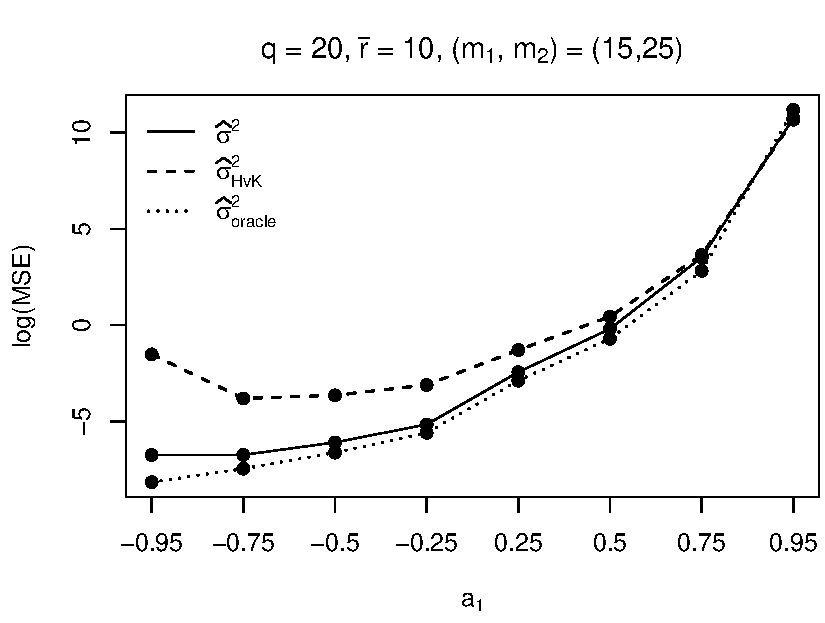
\includegraphics[width=\textwidth]{Plots/Robustness/MSE_lrv_T=500_slope=10_(q,r,M1,M2)=(20,10,15,25).pdf}
\end{subfigure}
\hspace{0.25cm}
\begin{subfigure}[b]{0.45\textwidth}
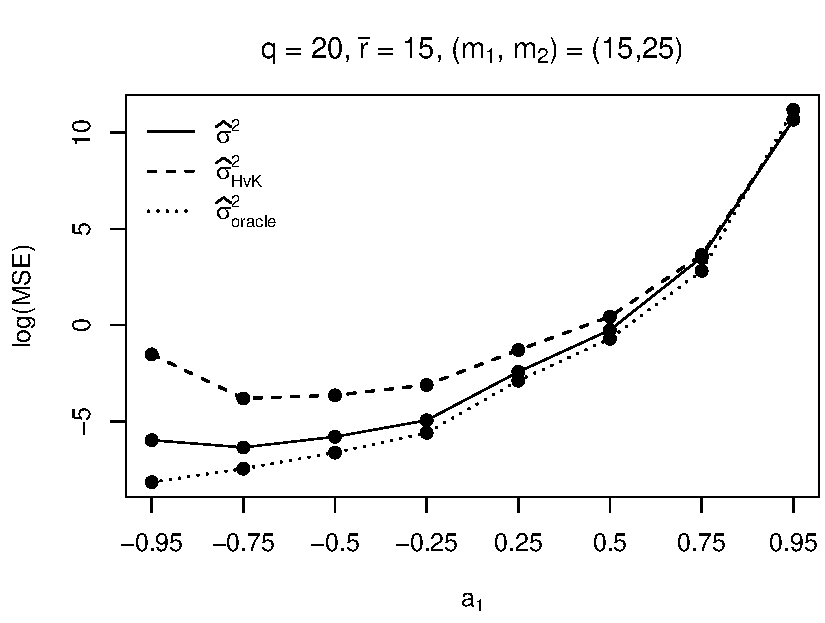
\includegraphics[width=\textwidth]{Plots/Robustness/MSE_lrv_T=500_slope=10_(q,r,M1,M2)=(20,15,15,25).pdf}
\end{subfigure}

\begin{subfigure}[b]{0.45\textwidth}
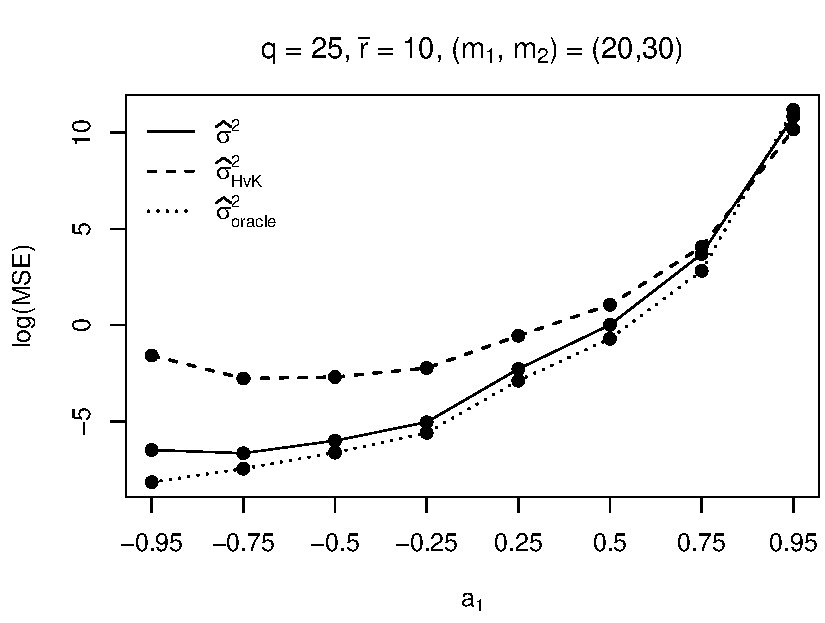
\includegraphics[width=\textwidth]{Plots/Robustness/MSE_lrv_T=500_slope=10_(q,r,M1,M2)=(25,10,20,30).pdf}
\end{subfigure}
\hspace{0.25cm}
\begin{subfigure}[b]{0.45\textwidth}
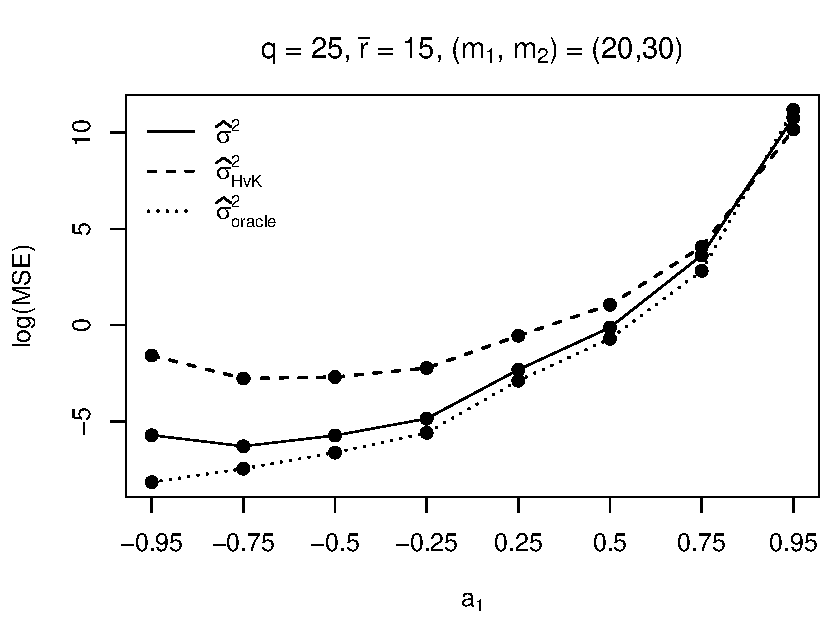
\includegraphics[width=\textwidth]{Plots/Robustness/MSE_lrv_T=500_slope=10_(q,r,M1,M2)=(25,15,20,30).pdf}
\end{subfigure}

\begin{subfigure}[b]{0.45\textwidth}
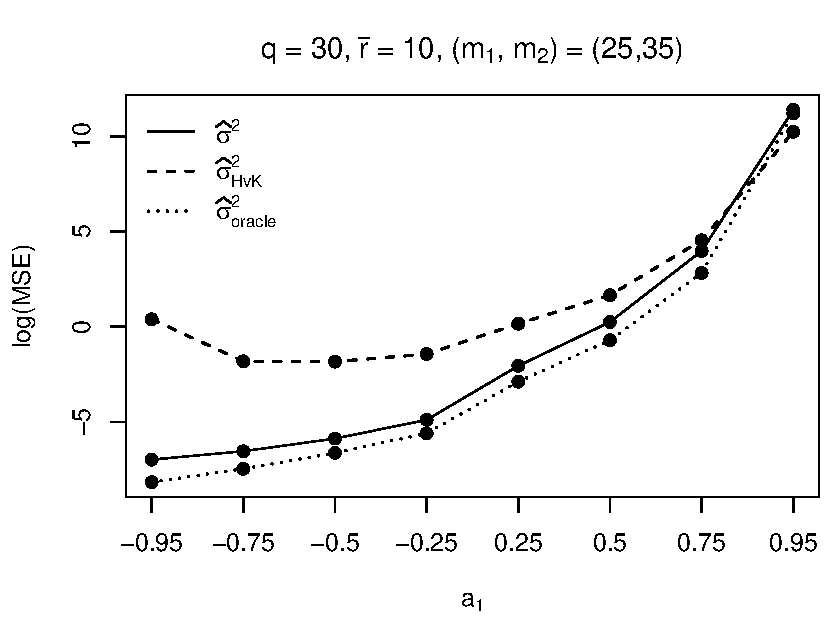
\includegraphics[width=\textwidth]{Plots/Robustness/MSE_lrv_T=500_slope=10_(q,r,M1,M2)=(30,10,25,35).pdf}
\end{subfigure}
\hspace{0.25cm}
\begin{subfigure}[b]{0.45\textwidth}
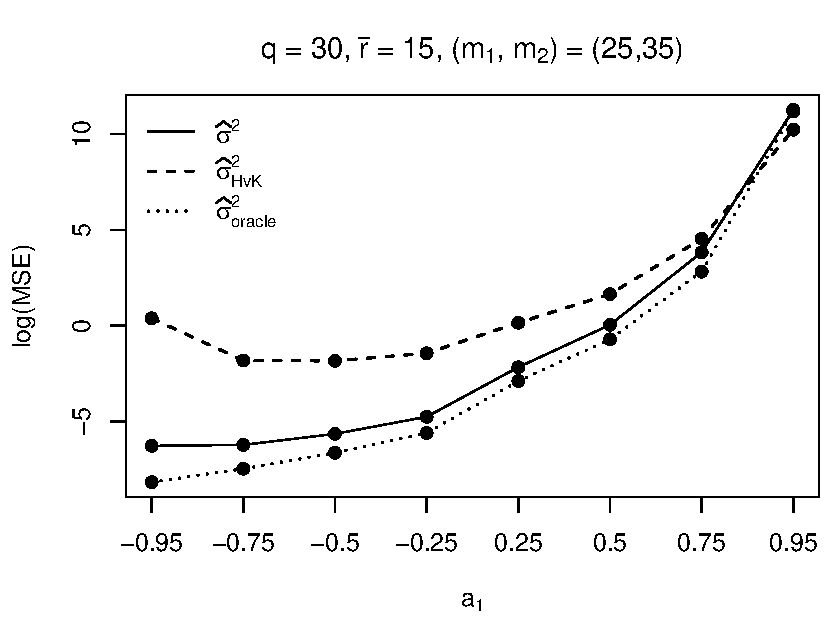
\includegraphics[width=\textwidth]{Plots/Robustness/MSE_lrv_T=500_slope=10_(q,r,M1,M2)=(30,15,25,35).pdf}
\end{subfigure}

\begin{subfigure}[b]{0.45\textwidth}
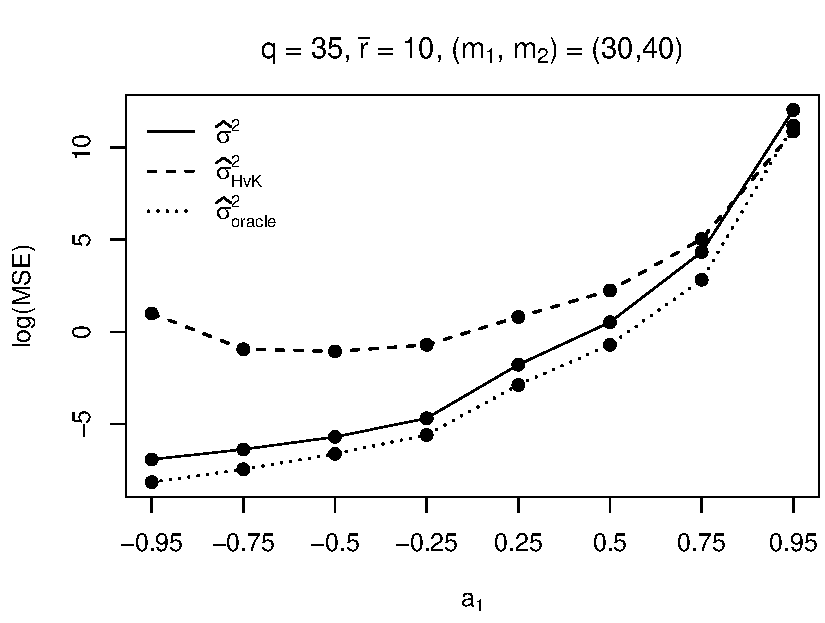
\includegraphics[width=\textwidth]{Plots/Robustness/MSE_lrv_T=500_slope=10_(q,r,M1,M2)=(35,10,30,40).pdf}
\end{subfigure}
\hspace{0.25cm}
\begin{subfigure}[b]{0.45\textwidth}
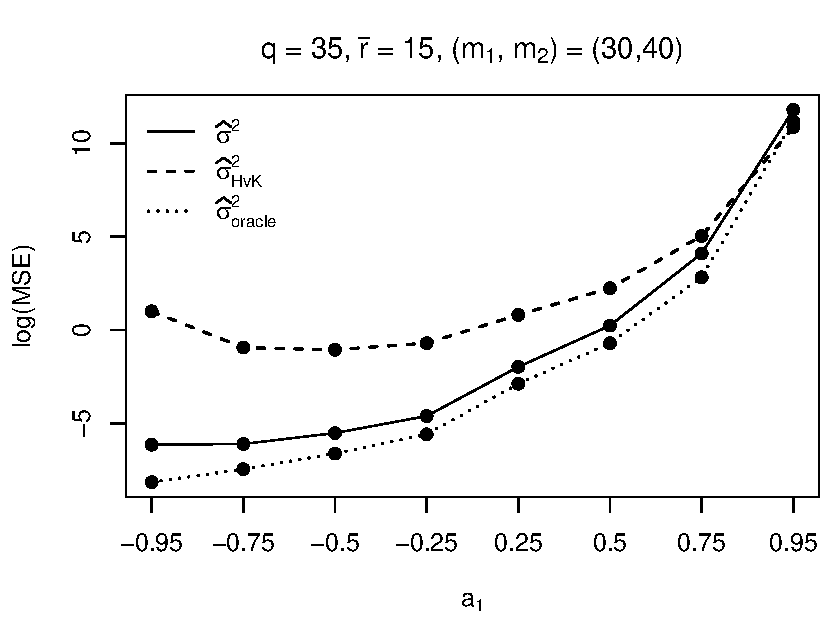
\includegraphics[width=\textwidth]{Plots/Robustness/MSE_lrv_T=500_slope=10_(q,r,M1,M2)=(35,15,30,40).pdf}
\end{subfigure}
\caption{Logarithmic MSE values for the estimators $\widehat{\sigma}^2$, $\widehat{\sigma}^2_{\text{HvK}}$ and $\widehat{\sigma}^2_{\text{oracle}}$ in the scenario with a pronounced trend ($s_\beta=10$).}\label{fig:MSE_slope10_lrv_robust} 
\end{figure}

